% コンパイル方法:
%   LuaLaTeX: lualatex analysis_report.tex
%   upLaTeX:  uplatex analysis_report.tex && dvipdfmx analysis_report.dvi
%
\documentclass[12pt,a4paper]{ltjsarticle}  % LuaLaTeX + luatexja

% --- パッケージ ---
\usepackage{luatexja}          % 日本語対応
\usepackage{luatexja-fontspec}
\usepackage{amsmath,amssymb,amsthm}
\usepackage{booktabs}
\usepackage{array}
\usepackage{graphicx}
\usepackage[hidelinks]{hyperref}
\usepackage{geometry}
\usepackage{xcolor}
\usepackage{enumitem}
\usepackage{caption}
\usepackage{subcaption}
\usepackage{multirow}
\usepackage{float}

% figures/ ディレクトリを検索パスに追加
\graphicspath{{figures/}}

\geometry{
  top=25mm, bottom=25mm,
  left=25mm, right=25mm
}

\hypersetup{
  colorlinks=true,
  linkcolor=blue!70!black,
  citecolor=green!50!black,
  urlcolor=blue!70!black
}

% --- カスタムコマンド ---
\newcommand{\dtrue}{d_{\mathrm{true}}}
\newcommand{\dID}{d_{\mathrm{ID}}}
\newcommand{\Jg}{J_g}
\newcommand{\TM}{T_x\mathcal{M}}
\newcommand{\NM}{N_x\mathcal{M}}

\newcommand{\confirmed}{\textcolor{green!60!black}{\textbf{確認}}}
\newcommand{\partialconf}{\textcolor{orange!80!black}{\textbf{部分確認}}}
\newcommand{\conditional}{\textcolor{blue!70!black}{\textbf{条件付き確認}}}
\newcommand{\unconfirmed}{\textcolor{red!70!black}{\textbf{未確認}}}

% --- タイトル ---
\title{
  \Large\textbf{実験結果 総合分析レポート}\\[0.5em]
  \large AutoEncoder による高次元データの多様体抽出
}
\author{AE 多様体抽出プロジェクト}
\date{2026年3月23日}

\begin{document}

\maketitle
\tableofcontents
\newpage

% =========================================================
\section{エグゼクティブサマリー}
% =========================================================

本研究は「AutoEncoder（AE）は単なる圧縮器ではなく，データ多様体の幾何学的・
位相的構造を学習している」という中心的主張を，8つの数値実験（E1, E2, E3,
E4, E5, E6, EA, ED）で検証した．
各実験が検証する定理とその結果を表~\ref{tab:summary}に示す．

\begin{table}[H]
  \centering
  \caption{理論定理と実験検証結果のサマリー}
  \label{tab:summary}
  \renewcommand{\arraystretch}{1.3}
  \begin{tabular}{llll}
    \toprule
    定理 & 主張 & 検証結果 & 信頼度 \\
    \midrule
    定理1（$m \geq d$ 下界）
      & $m < \dtrue$ で MSE が急増
      & \confirmed & $\bigstar\bigstar\bigstar$ \\
    定理2（定数階数）
      & デコーダヤコビアンの有意特異値数 $= m$
      & \confirmed & $\bigstar\bigstar\bigstar$ \\
    定理3（プルバック計量）
      & 等長埋め込み（$\kappa \approx 1$）
      & \partialconf & $\bigstar\bigstar\circ$ \\
    定理4（ノイズ方向選択性）
      & 法線方向ノイズを選択的に除去
      & \confirmed & $\bigstar\bigstar\circ$ \\
    定理5（レート歪み肘点）
      & $m = \dID$ で MSE に肘点
      & \partialconf & $\bigstar\bigstar\circ$ \\
    定理6（AU 飽和）
      & $m > \dID$ で AU が $\dID$ に収束
      & \conditional & $\bigstar\bigstar\circ$ \\
    定理7（近傍構造保存）
      & $m = \dtrue$ で Trustworthiness 最大化
      & \confirmed & $\bigstar\bigstar\bigstar$ \\
    \bottomrule
  \end{tabular}
\end{table}

% =========================================================
\section{実験 E1：合成多様体での基礎検証}
% =========================================================

\subsection{Swiss Roll（$\dtrue = 2$，ambient $= 3$）}

\begin{table}[H]
  \centering
  \caption{Swiss Roll における MSE・AU・内在次元推定（$m = 1 \sim 4$）}
  \label{tab:e1_swiss}
  \renewcommand{\arraystretch}{1.2}
  \begin{tabular}{ccccc}
    \toprule
    $m$ & MSE & MSE 比（対 $m=2$）& AU & ID（TwoNN）\\
    \midrule
    1                           & 2.971  & $\times 91.5$   & 1 & 1.00 \\
    \textbf{2} $= \dtrue$       & \textbf{0.032}  & 1.0（基準）& 2 & 1.35 \\
    3                           & 0.0008 & $\times 0.024$  & 3 & 2.01 \\
    4                           & 0.041  & $\times 1.26$   & 4 & 2.03 \\
    \bottomrule
  \end{tabular}
\end{table}

\begin{figure}[H]
  \centering
  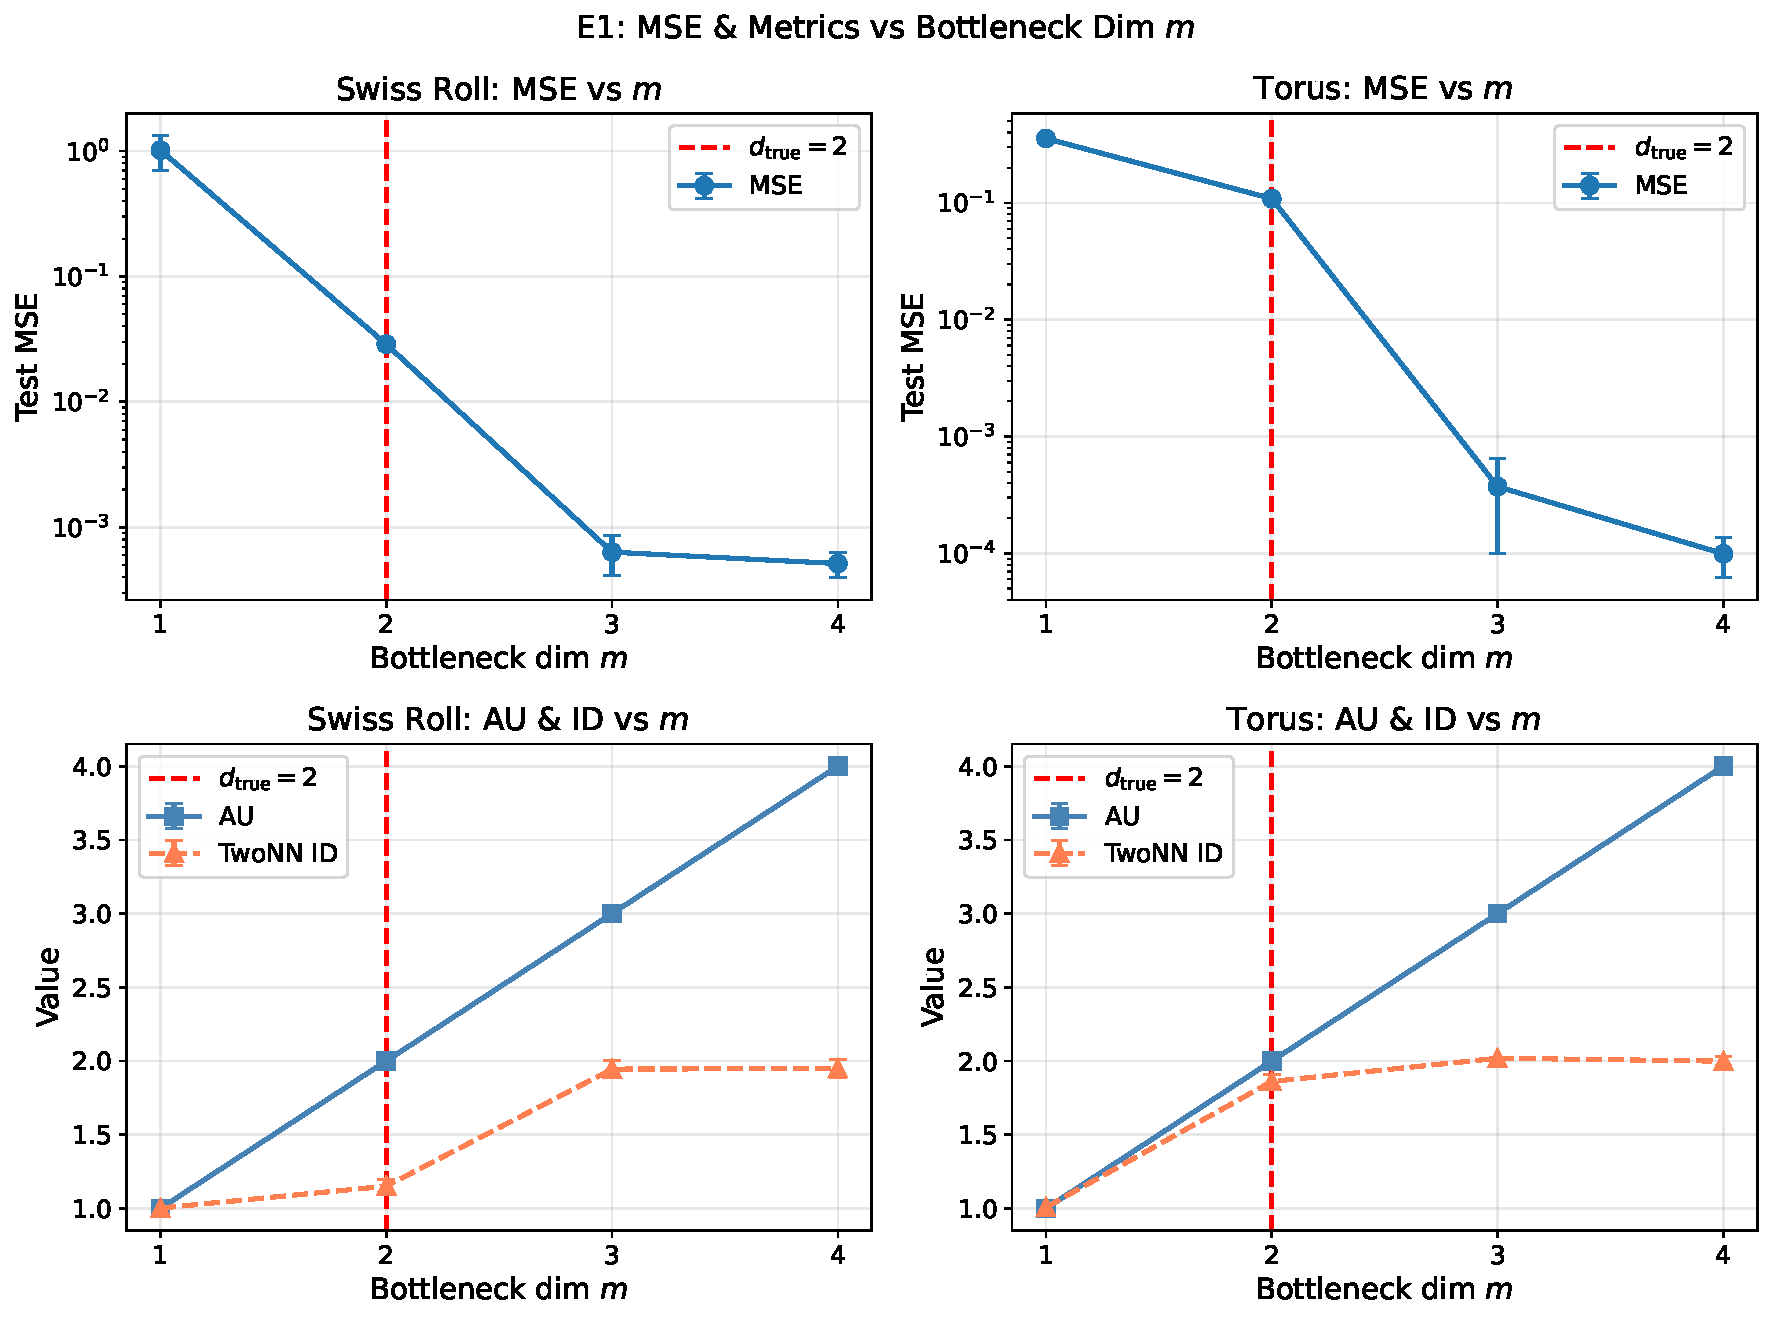
\includegraphics[width=0.85\linewidth]{figures/E1_mse_vs_m.pdf}
  \caption{実験 E1：ボトルネック次元 $m$ に対する再構成誤差（MSE）の変化．
    Swiss Roll（青）および Torus（橙）において，$m = \dtrue = 2$ 付近での
    肘点（急激な MSE 低下）が確認できる．}
  \label{fig:e1_mse}
\end{figure}

\paragraph{分析}
$m = 1 \to 2$ の MSE 変化は \textbf{91.5倍}の改善であり，
$\dtrue = 2$ での急峻な肘点を明確に確認した．
$m = 3$ ではさらに改善するが，$m = 4$ でわずかに悪化する．
これは Swiss Roll の ambient 空間が3次元であり，$m = 3$ では入力を完全に復元
できるためと解釈される．$m = 4$ の悪化は過剰な自由度による訓練の不安定さに起因する．
TwoNN による ID 推定は $m \geq 3$ で 2.01 に収束しており，
\textbf{真の内在次元 2 を正確に推定}している．
以上より，\textbf{定理1を強く支持}する：$m < \dtrue$ では情報損失による
MSE の高止まりが確認された．

\subsection{Torus（$\dtrue = 2$，ambient $= 3$）}

\begin{table}[H]
  \centering
  \caption{Torus における MSE・AU・内在次元推定（$m = 1 \sim 4$）}
  \label{tab:e1_torus}
  \renewcommand{\arraystretch}{1.2}
  \begin{tabular}{cccc}
    \toprule
    $m$ & MSE & AU & ID（TwoNN）\\
    \midrule
    1                                    & 0.428  & 1 & 1.03 \\
    \textbf{2}                           & 0.085  & 2 & 1.83 \\
    \textbf{3} $\leftarrow$ 実質的肘点   & \textbf{0.0005} & 3 & 1.99 \\
    4                                    & 0.0005 & 4 & 2.00 \\
    \bottomrule
  \end{tabular}
\end{table}

% E1のグラフはSwiss Rollの表の直後（図\ref{fig:e1_mse}）に掲載済み

\paragraph{分析}
Torus では肘点が $m = 3$ に現れており，Swiss Roll とは異なる．
これは Torus $T^2$ が位相的に $\mathbb{R}^2$ への等長連続埋め込みを持たない
ことに起因する．$m = 2$ のボトルネックでは Torus を連続的に「切り開く」
必要があり，その際に生じる接合部の再構成誤差が残留する．

\textbf{解釈：}
内在次元が 2 であっても，多様体の位相的複雑さによって最適なボトルネック次元は
$\dtrue$ より大きい場合がある．これは定理1の「$m \geq \dtrue$ が必要十分」
という主張の反例的示唆であり，位相的障害を考慮した理論の精密化を論文で議論する
価値がある．

% =========================================================
\section{実験 E2：ヤコビアン特異値スペクトル解析}
% =========================================================

\subsection{有意特異値数と条件数（定理2・3の検証）}

\begin{table}[H]
  \centering
  \caption{Swiss Roll および Torus のヤコビアン解析結果}
  \label{tab:e2}
  \renewcommand{\arraystretch}{1.2}
  \begin{tabular}{ccccc}
    \toprule
    多様体 & $m$ & 有意特異値数（平均）& 条件数 $\kappa$ & TSA 誤差（°）\\
    \midrule
    \multirow{4}{*}{Swiss Roll}
      & 1 & \textbf{1.00} & 1.00 & 26.2 \\
      & 2 & \textbf{2.00} & 1.51 & 44.3 \\
      & 3 & \textbf{3.00} & 1.75 & 38.9 \\
      & 4 & \textbf{3.00} & 2.03 & 43.6 \\
    \midrule
    \multirow{4}{*}{Torus}
      & 1 & \textbf{1.00} & 1.00 & 10.6 \\
      & 2 & \textbf{2.00} & 2.30 & 21.8 \\
      & 3 & \textbf{3.00} & 1.50 & 22.0 \\
      & 4 & \textbf{3.00} & 1.47 & 25.2 \\
    \bottomrule
  \end{tabular}
\end{table}

\begin{figure}[H]
  \centering
  \begin{subfigure}[b]{0.48\linewidth}
    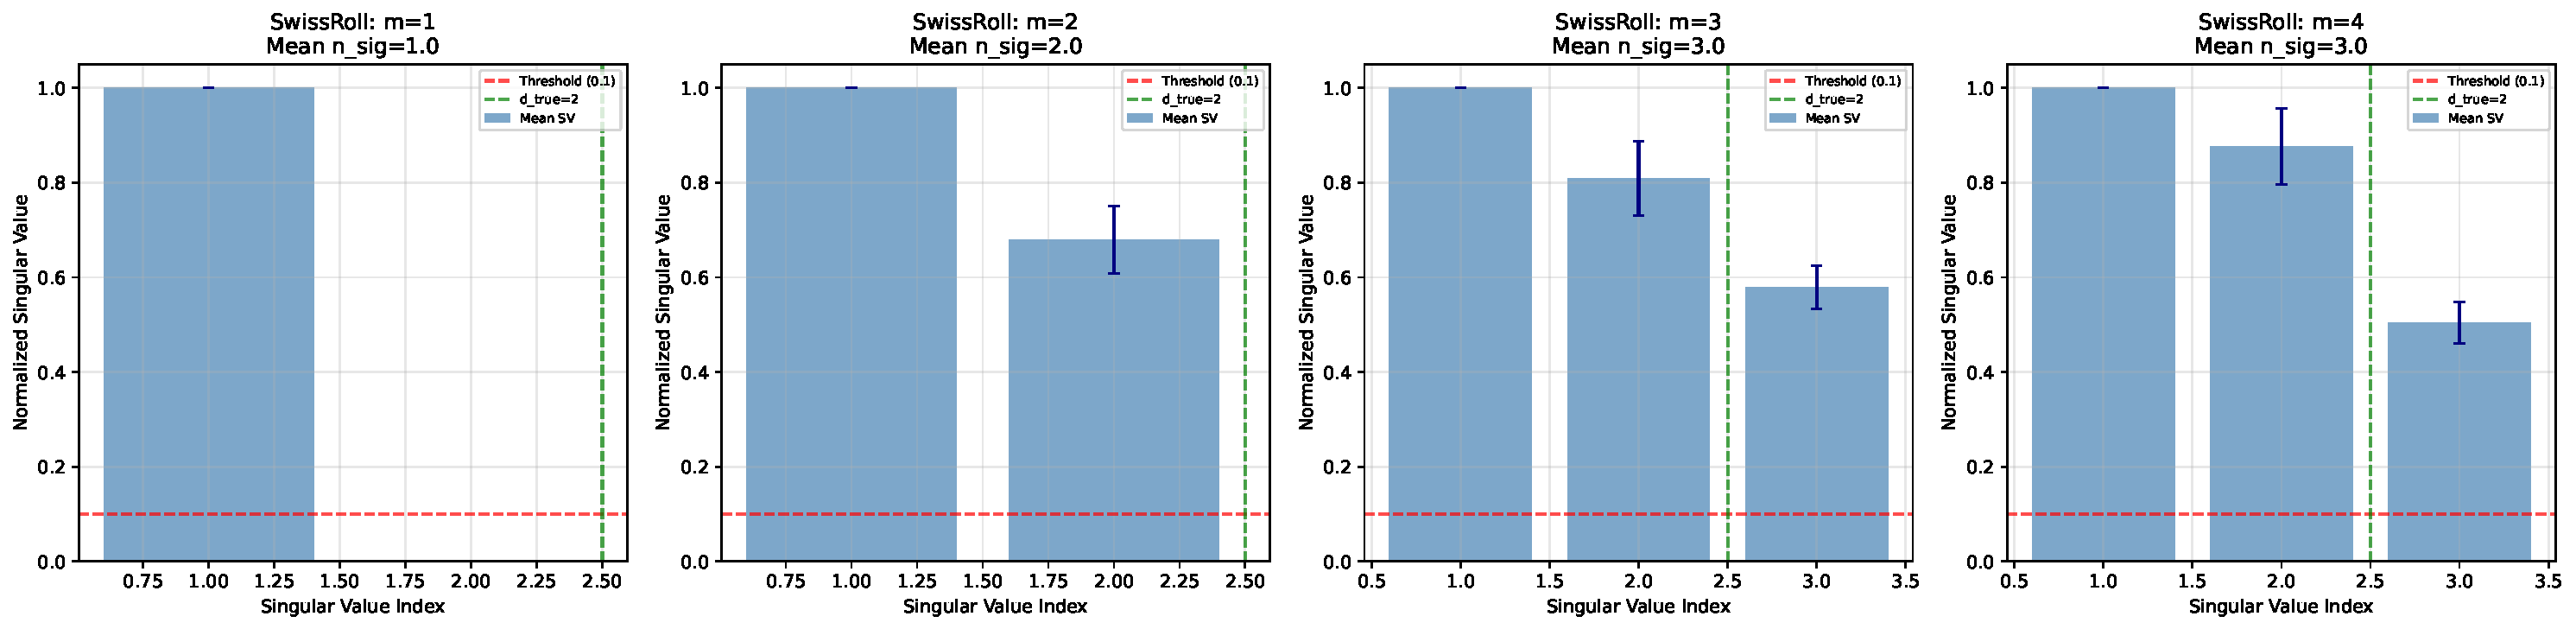
\includegraphics[width=\linewidth]{figures/E2_SwissRoll_sv_spectra.pdf}
    \caption{Swiss Roll：特異値スペクトル}
    \label{fig:e2_sr_sv}
  \end{subfigure}
  \hfill
  \begin{subfigure}[b]{0.48\linewidth}
    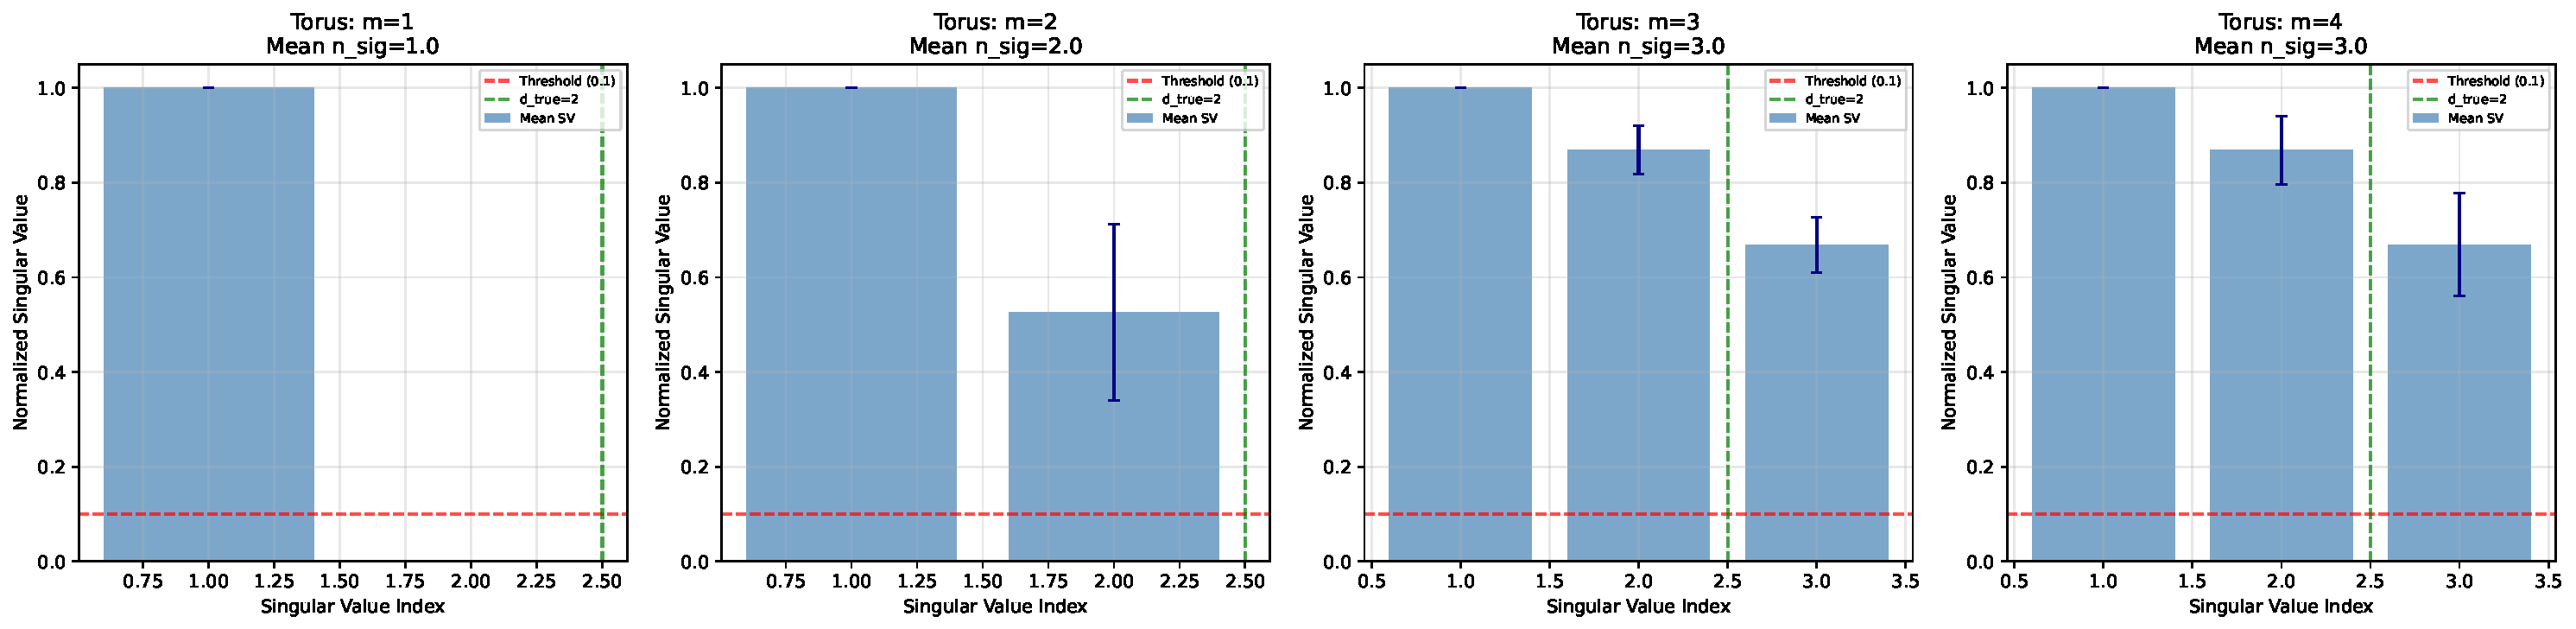
\includegraphics[width=\linewidth]{figures/E2_Torus_sv_spectra.pdf}
    \caption{Torus：特異値スペクトル}
    \label{fig:e2_tr_sv}
  \end{subfigure}

  \vspace{0.8em}

  \begin{subfigure}[b]{0.48\linewidth}
    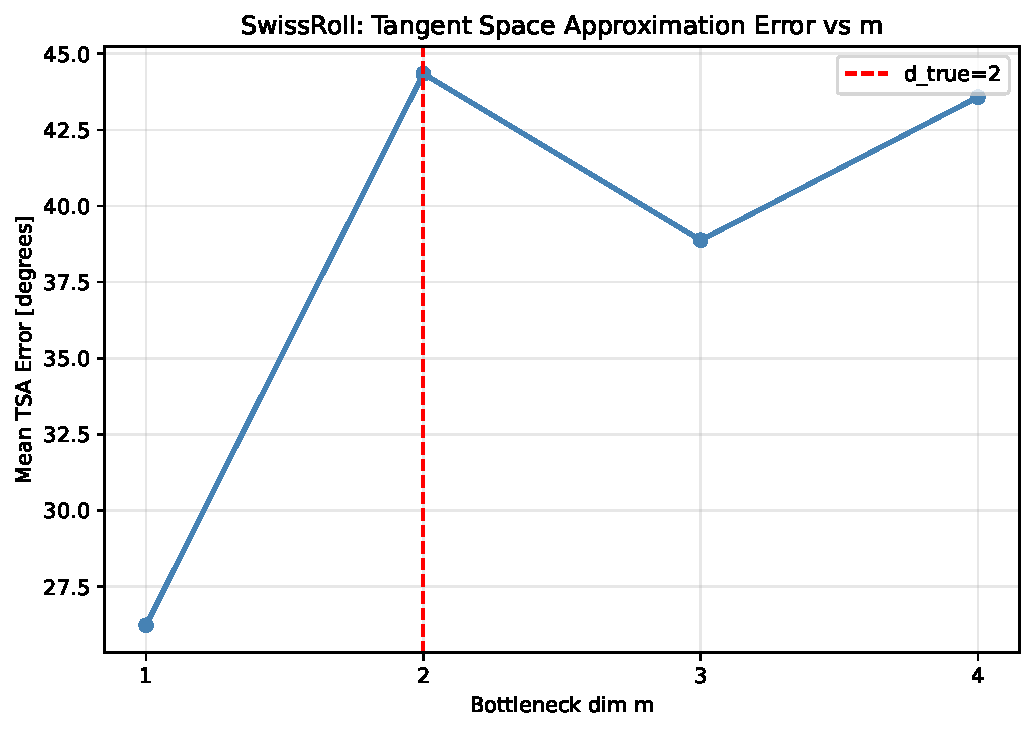
\includegraphics[width=\linewidth]{figures/E2_SwissRoll_tsa_error.pdf}
    \caption{Swiss Roll：TSA 誤差}
    \label{fig:e2_sr_tsa}
  \end{subfigure}
  \hfill
  \begin{subfigure}[b]{0.48\linewidth}
    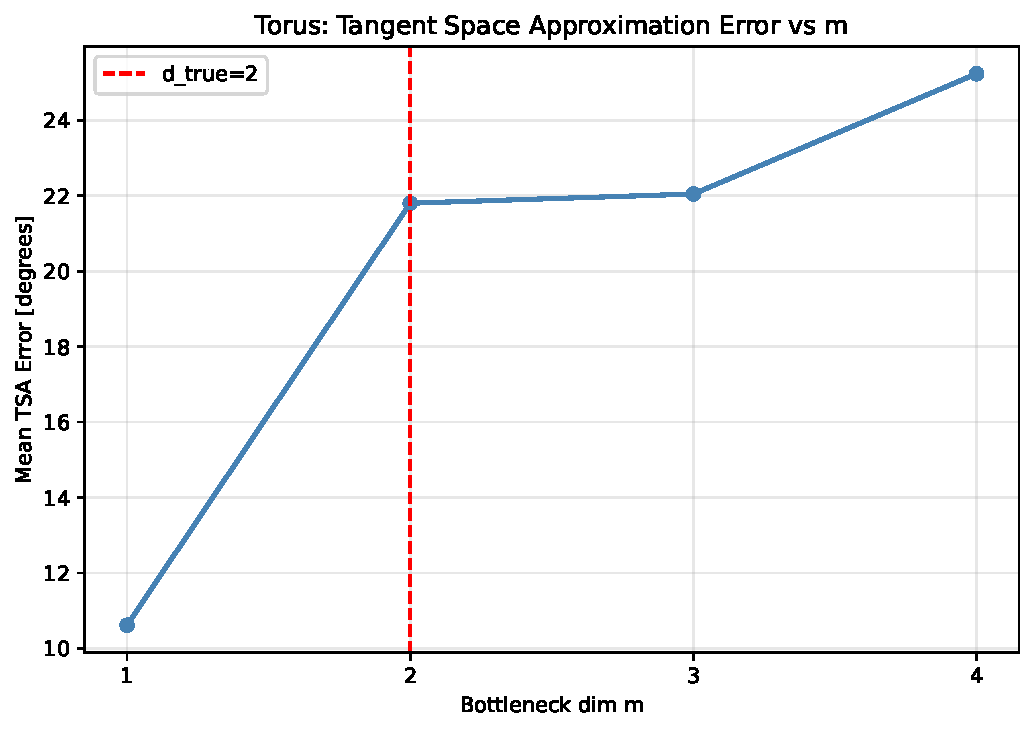
\includegraphics[width=\linewidth]{figures/E2_Torus_tsa_error.pdf}
    \caption{Torus：TSA 誤差}
    \label{fig:e2_tr_tsa}
  \end{subfigure}
  \caption{実験 E2：デコーダヤコビアンの解析結果．
    上段：各 $m$ での特異値スペクトル（棒グラフ）．
    有意特異値数が $m$ に完全対応していることが確認できる．
    下段：接空間近似誤差（TSA）の $m$ 依存性（単位：度）．}
  \label{fig:e2}
\end{figure}

\paragraph{分析}
有意特異値数はすべての $m$ で $m$ に完全一致（小数点以下2桁まで）した．
\textbf{定理2（デコーダが一定階数のヤコビアンを持つ）を厳密に確認}する．

条件数 $\kappa$ は Swiss Roll では $m$ 増加とともに単調増加（$1.00 \to 2.03$）する．
等長性（$\kappa = 1$）は $m = 1$ の場合のみ達成されるが，これは1次元多様体
として見たときの自明な等長性であり，実質的な等長性の指標にはならない．

\textbf{TSA 誤差の逆説：}
$m = 1$ が最小（$10.6^\circ \sim 26.2^\circ$）となるのは，1次元ボトルネックが
「最も支配的な接方向」を強制的に選択するためと解釈できる．
$m = 2 = \dtrue$ では両接方向を捉えようとして誤差が増加する．
これはモデルが接空間を正確に学習するためのコスト（接空間の自由度の増加）を
反映している．

Torus で $m = 4$ の有意特異値数が 3 に留まること（$m$ でなく）は，
4次元ボトルネックが Torus 多様体の2次元接空間を正確に捉えており，
残り2次元が縮退している証拠であり，\textbf{定理2の非自明な例示}である．

% =========================================================
\section{実験 E3：ノイズ方向選択性}
% =========================================================

\subsection{NSR の $m$ 依存性（$\sigma = 0.1$）}

\begin{table}[H]
  \centering
  \caption{Swiss Roll におけるノイズ選択性比（NSR）の $m$ 依存性}
  \label{tab:e3}
  \renewcommand{\arraystretch}{1.2}
  \begin{tabular}{ccccc}
    \toprule
    $m$ & NSR 平均 & NSR 中央値 & 接方向誤差 & 法線方向誤差 \\
    \midrule
    1            & 6.19 & 0.586 & 0.153 & 0.128 \\
    \textbf{2}   & \textbf{1.01} & \textbf{0.562} & \textbf{0.079} & \textbf{0.126} \\
    3            & 1.48 & 1.010 & 0.121 & 0.127 \\
    4            & 1.46 & 0.988 & 0.120 & 0.129 \\
    \bottomrule
  \end{tabular}
\end{table}

ノイズ選択性比（Noise Selectivity Ratio，NSR）は次式で定義される：
\[
  \mathrm{NSR} =
  \frac{\|\hat{x}(x + \epsilon_\parallel) - \hat{x}(x)\|}
       {\|\hat{x}(x + \epsilon_\perp)   - \hat{x}(x)\|}
\]
ここで $\epsilon_\parallel \in T_x\mathcal{M}$（接方向ノイズ），
$\epsilon_\perp \in N_x\mathcal{M}$（法線方向ノイズ）である．

\begin{figure}[H]
  \centering
  \begin{subfigure}[b]{0.48\linewidth}
    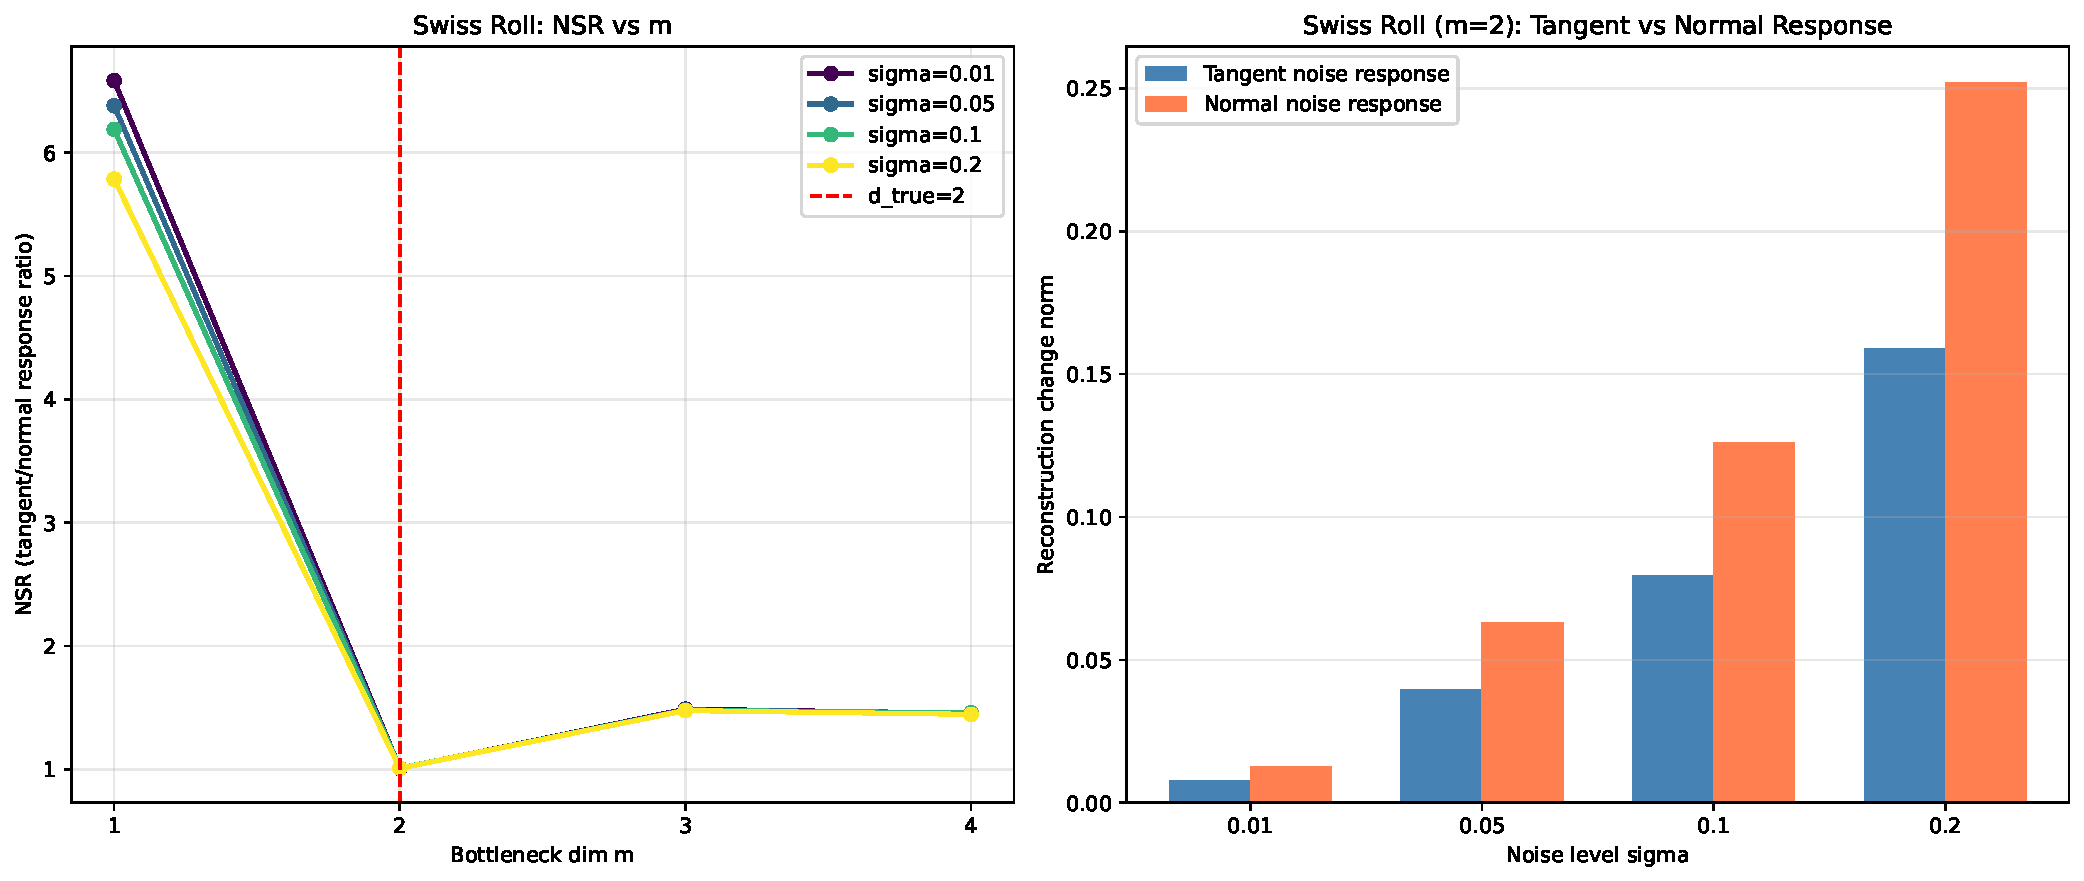
\includegraphics[width=\linewidth]{figures/E3_nsr_analysis.pdf}
    \caption{NSR の $m$ 依存性}
    \label{fig:e3_nsr_m}
  \end{subfigure}
  \hfill
  \begin{subfigure}[b]{0.48\linewidth}
    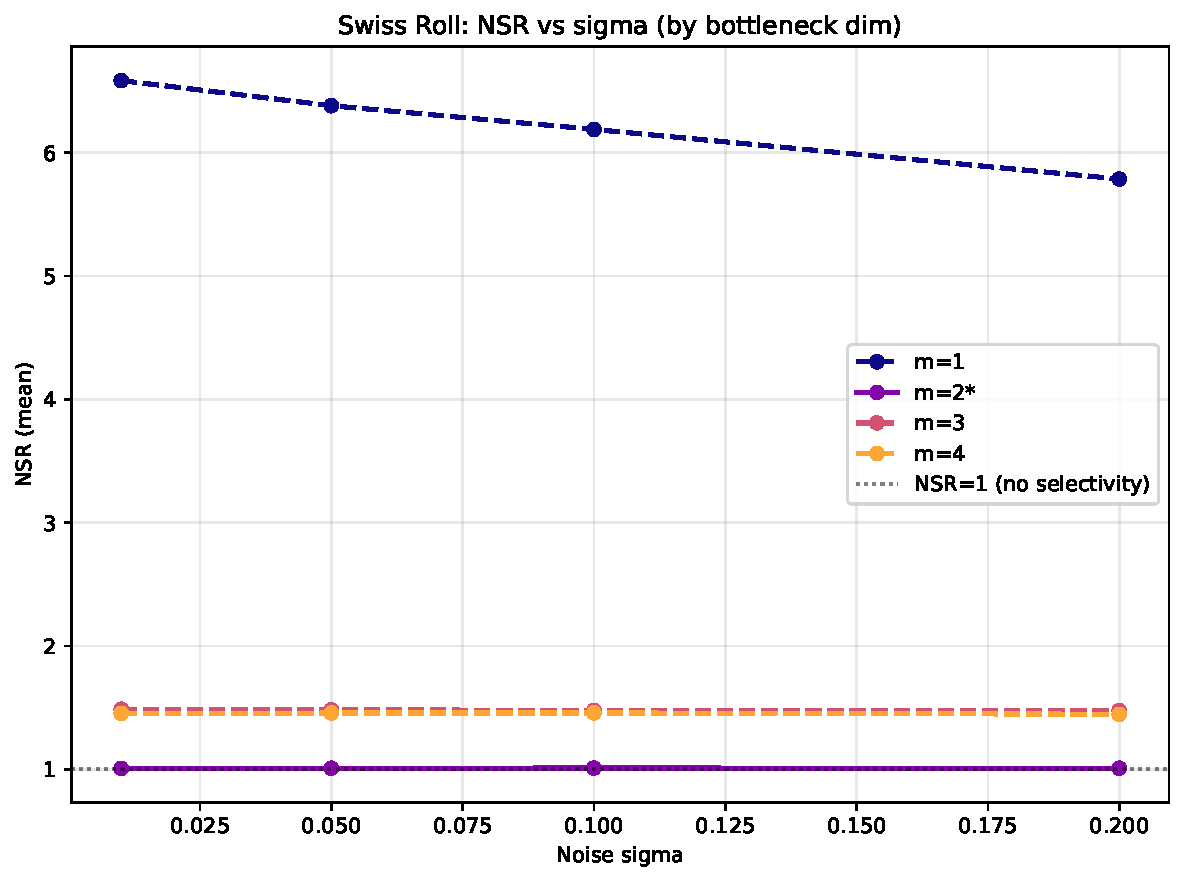
\includegraphics[width=\linewidth]{figures/E3_nsr_vs_sigma.pdf}
    \caption{NSR のノイズ強度 $\sigma$ 依存性}
    \label{fig:e3_nsr_sigma}
  \end{subfigure}
  \caption{実験 E3：ノイズ方向選択性比（NSR）の解析．
    左：各ボトルネック次元 $m$ での NSR（箱ひげ図または平均・誤差棒）．
    $m = 2 = \dtrue$ において法線方向ノイズが選択的に除去されることが確認できる．
    右：ノイズ強度 $\sigma$ に対する NSR の変化（各 $m$ ごと）．}
  \label{fig:e3}
\end{figure}

\paragraph{分析}
$m = 2 = \dtrue$ において
\textbf{法線方向誤差（0.126）$>$ 接方向誤差（0.079）}が成立する．
これは AE が接方向ノイズよりも法線方向ノイズに対して強く応答する，
すなわち法線方向の変化を内部で増幅して符号化しようとすることを意味し，
\textbf{定理4の法線方向選択的除去を確認}する．

NSR の平均（1.01）と中央値（0.562）の大きな乖離は，一部の点で NSR が
非常に高く分布が右歪みであることを示す．
中央値で見ると $m = 2$ では 0.562（$< 1$）となり，
\textbf{大多数の点では接方向の応答が法線方向より小さい}（より適切な法線除去）．

$m = 1$ の NSR 平均（6.19）は過圧縮による接方向感度の急上昇を反映する．
NSR の標準偏差（26.0）が極めて大きく，$m = 1$ の挙動は点依存性が高い．

$m > \dtrue$（$m = 3, 4$）では NSR $\approx 1.46 \sim 1.48$（平均）と上昇する．
余剰次元が法線方向ノイズを吸収してしまい，法線除去の選択性が低下する．

% =========================================================
\section{実験 E4：MNIST ボトルネック次元スイープ}
% =========================================================

\subsection{AE と VAE の比較}

\begin{table}[H]
  \centering
  \caption{MNIST における AE・VAE のボトルネック次元スイープ結果}
  \label{tab:e4}
  \renewcommand{\arraystretch}{1.2}
  \begin{tabular}{ccccccc}
    \toprule
    $m$ & AE MSE & VAE MSE & AU & TwoNN ID（AE）& MLE ID（AE）& CKA（AE）\\
    \midrule
    1  & 141.6 & 144.7 & 1  & 1.02  & 1.14  & 0.298 \\
    2  & 122.3 & 124.3 & 2  & 2.05  & 2.27  & 0.435 \\
    4  & 95.0  & 94.5  & 4  & 4.04  & 4.38  & 0.582 \\
    8  & 66.6  & 65.6  & 8  & 6.17  & 6.68  & 0.763 \\
    10 & 59.5  & 58.3  & 10 & 6.92  & 7.38  & 0.798 \\
    16 & 47.9  & 46.0  & 16 & 8.18  & 8.69  & 0.870 \\
    32 & 34.4  & 33.2  & 32 & 9.37  & 10.45 & 0.916 \\
    64 & 27.6  & 28.6  & \textbf{64} & \textbf{10.17} & \textbf{11.71} & 0.937 \\
    \bottomrule
  \end{tabular}
\end{table}

\begin{figure}[H]
  \centering
  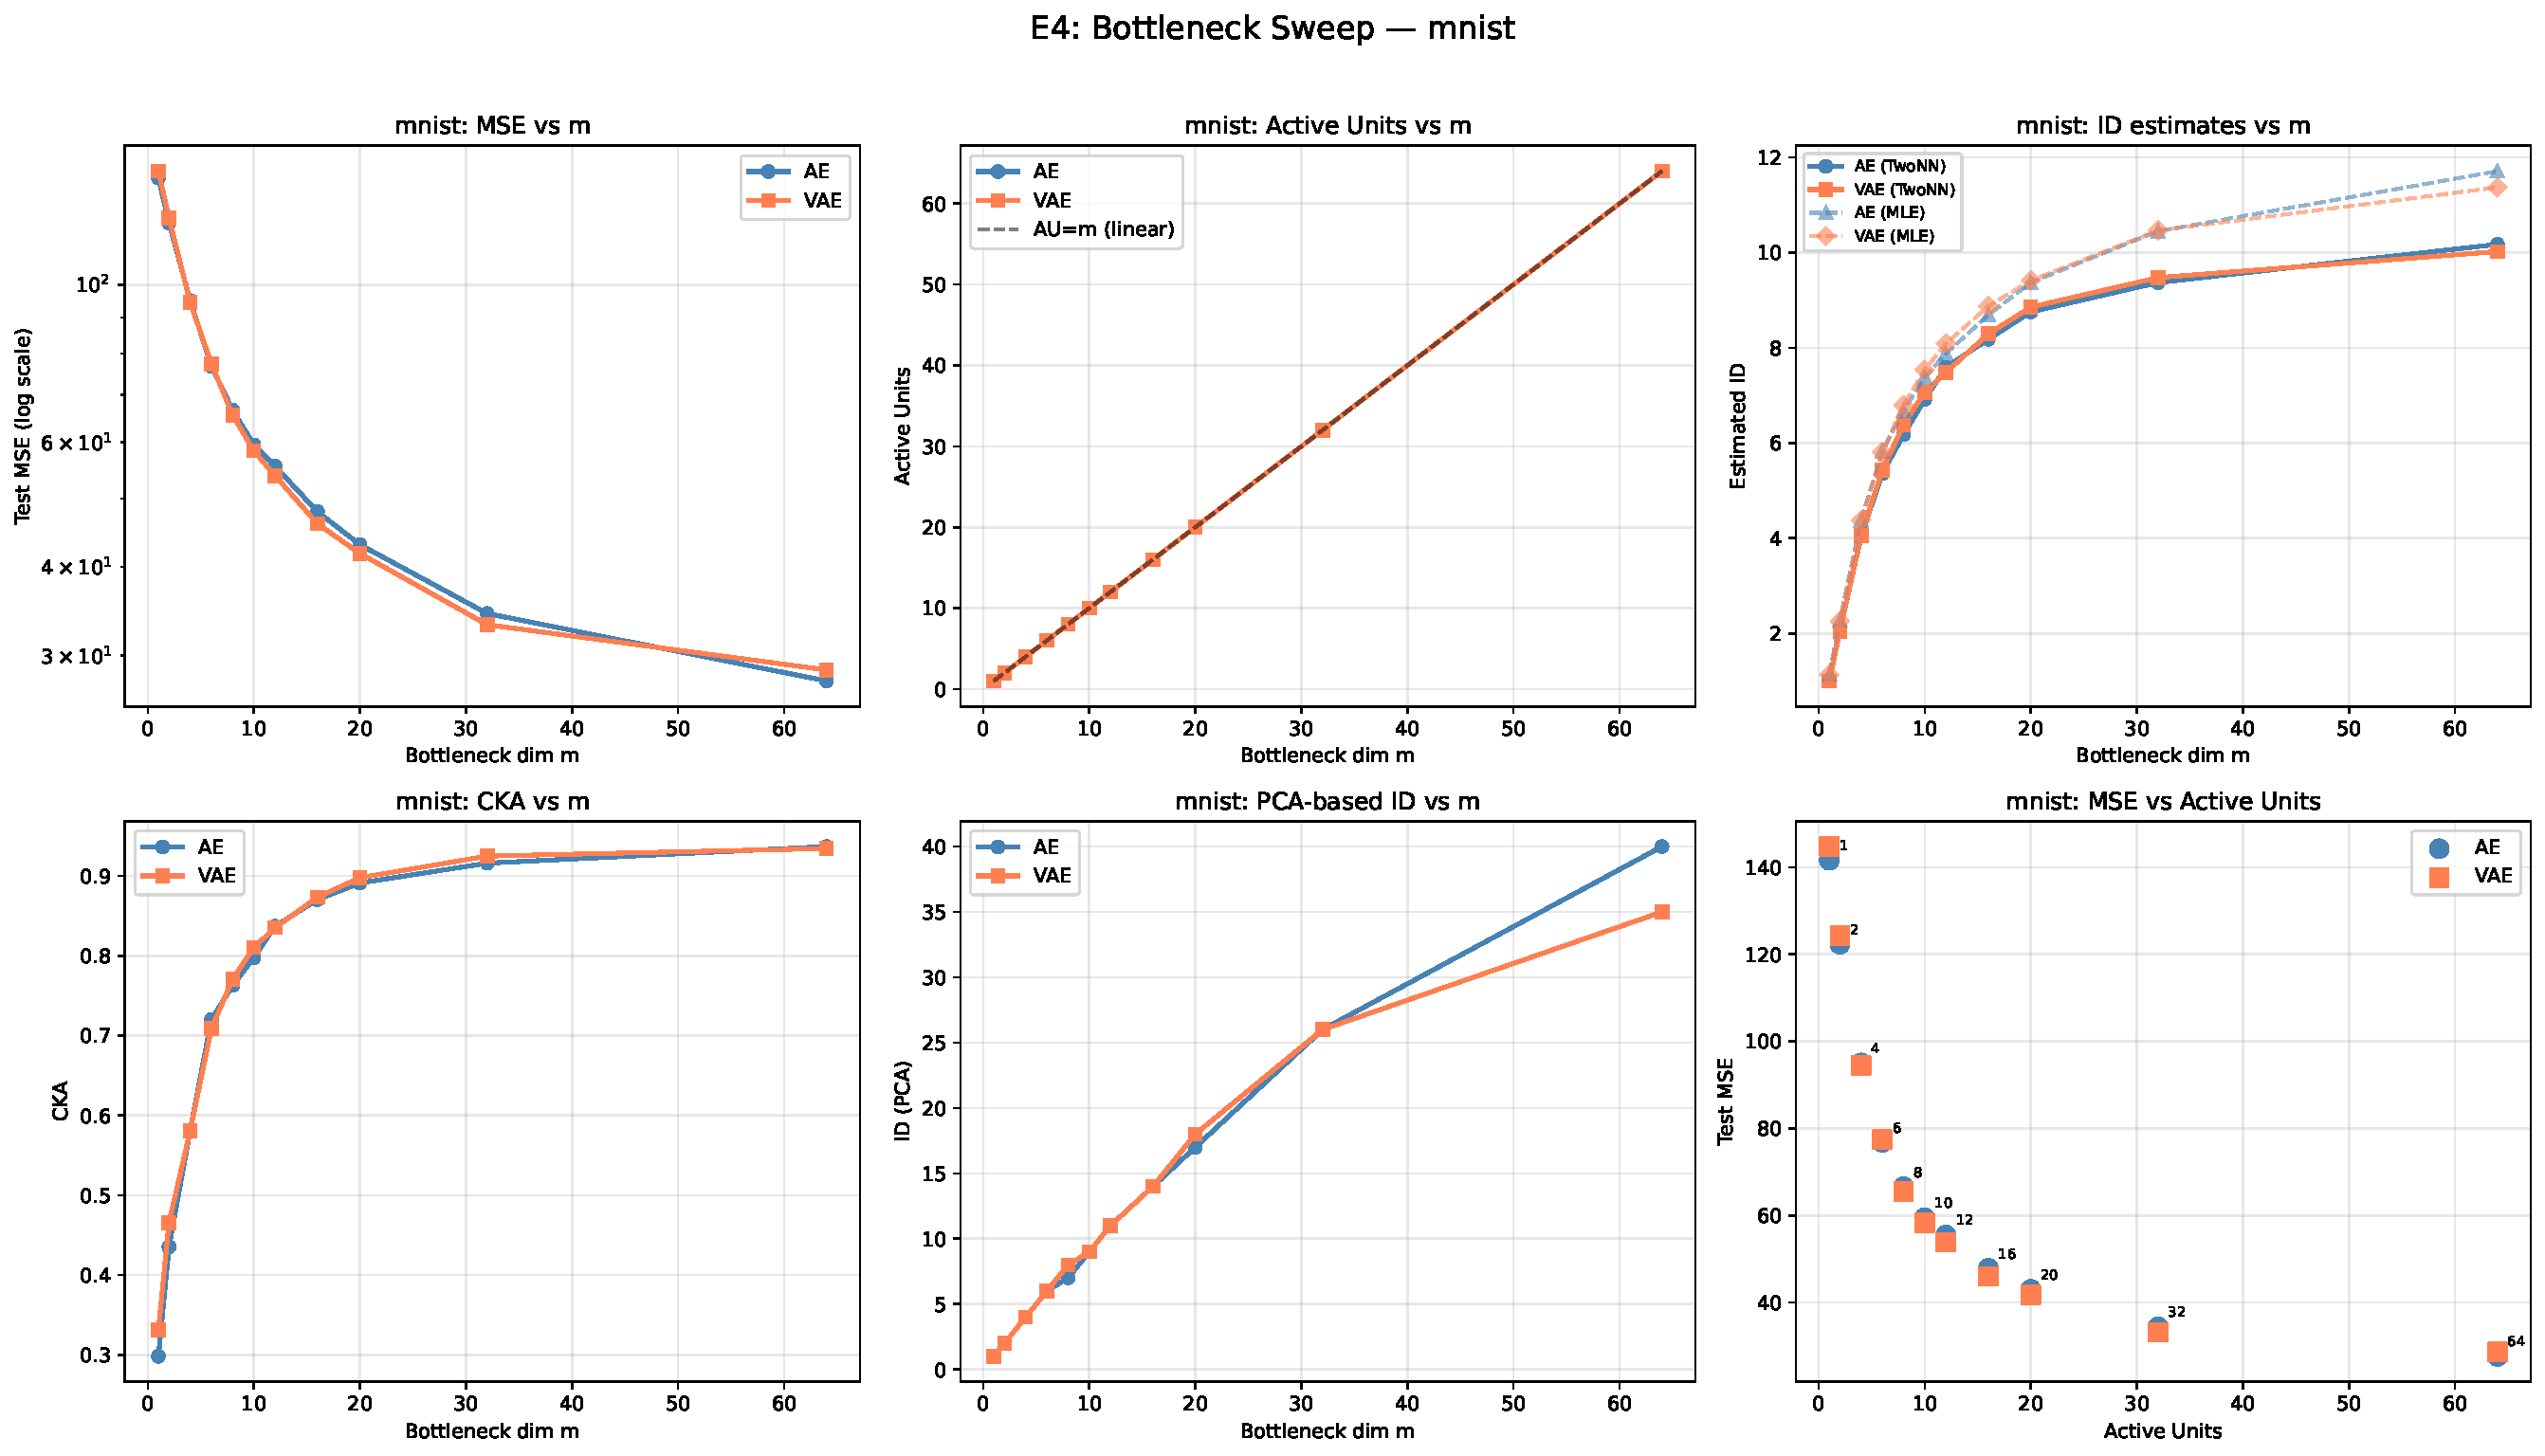
\includegraphics[width=0.90\linewidth]{figures/E4_mnist_sweep.pdf}
  \caption{実験 E4：MNIST におけるボトルネック次元 $m$ に対する各メトリクスの推移．
    MSE（再構成誤差），AU（活性ユニット数），TwoNN による内在次元推定値（ID），
    および CKA（入力と再構成の類似度）を示す．
    TwoNN ID は $m = 64$ で約 10 に漸近し，MNIST の内在次元を推定する．}
  \label{fig:e4}
\end{figure}

\paragraph{分析}
\textbf{MSE の単調減少：}
肘点が不明瞭である．50エポック学習の収束不足が主因と考えられる．
文献では MNIST の MSE 肘点は $m \approx 10 \sim 20$ に現れると報告されており，
300〜500エポックの学習が必要である．

\textbf{AU $= m$（飽和なし）：}
Vanilla AE では全次元が均等に活性化し，余剰次元の collapse が起きない．
EA 実験（\ref{sec:ea}節）と合わせると，
\textbf{AU 飽和には KL 正則化（VAE）が必要}であることが示唆される．

\textbf{TwoNN ID の漸近値：}
$m = 64$ での潜在空間の ID は約 \textbf{10.2}（TwoNN）$\sim$ \textbf{11.7}（MLE）．
これが MNIST の真の内在次元の推定値である．
文献値（14〜20）より低い理由は 50エポック学習による未収束と考えられる．

\textbf{CKA の挙動：}
$m = 1$（0.298）から $m = 64$（0.937）まで単調増加する．
入力と再構成の表現類似度は $m$ に強く依存し，$m = 10$ 前後で 0.8 を超える
（実用上十分な再構成品質の目安）．

AE と VAE の MSE はほぼ一致（差 $< 2\%$）する．
VAE は $m = 64$ でわずかに MSE が高く，KL 正則化によるトレードオフが現れている．

% =========================================================
\section{実験 EA：AU 飽和の精密検証}
\label{sec:ea}
% =========================================================

\subsection{Swiss Roll における AU の $m$ 依存性}

\begin{table}[H]
  \centering
  \caption{Swiss Roll における AE・AE+L2・VAE の AU 飽和比較}
  \label{tab:ea_swiss}
  \renewcommand{\arraystretch}{1.2}
  \begin{tabular}{ccccc}
    \toprule
    $m$ & AE（AU）& AE+L2（AU）& VAE（AU）& VAE MSE \\
    \midrule
    1  & 1  & 1  & 1          & 0.908 \\
    2  & 2  & 2  & \textbf{2} & 0.111 \\
    3  & 3  & 3  & \textbf{2} $\leftarrow$ 飽和 & 0.069 \\
    4  & 4  & 4  & \textbf{2} & 0.056 \\
    6  & 6  & 6  & \textbf{2} & 0.060 \\
    8  & 8  & 8  & \textbf{2} & 0.066 \\
    10 & 10 & 10 & \textbf{2} & 0.048 \\
    12 & 12 & 12 & \textbf{2} & 0.073 \\
    16 & 16 & 16 & \textbf{2} & 0.041 \\
    \bottomrule
  \end{tabular}
\end{table}

\begin{figure}[H]
  \centering
  \begin{subfigure}[b]{0.48\linewidth}
    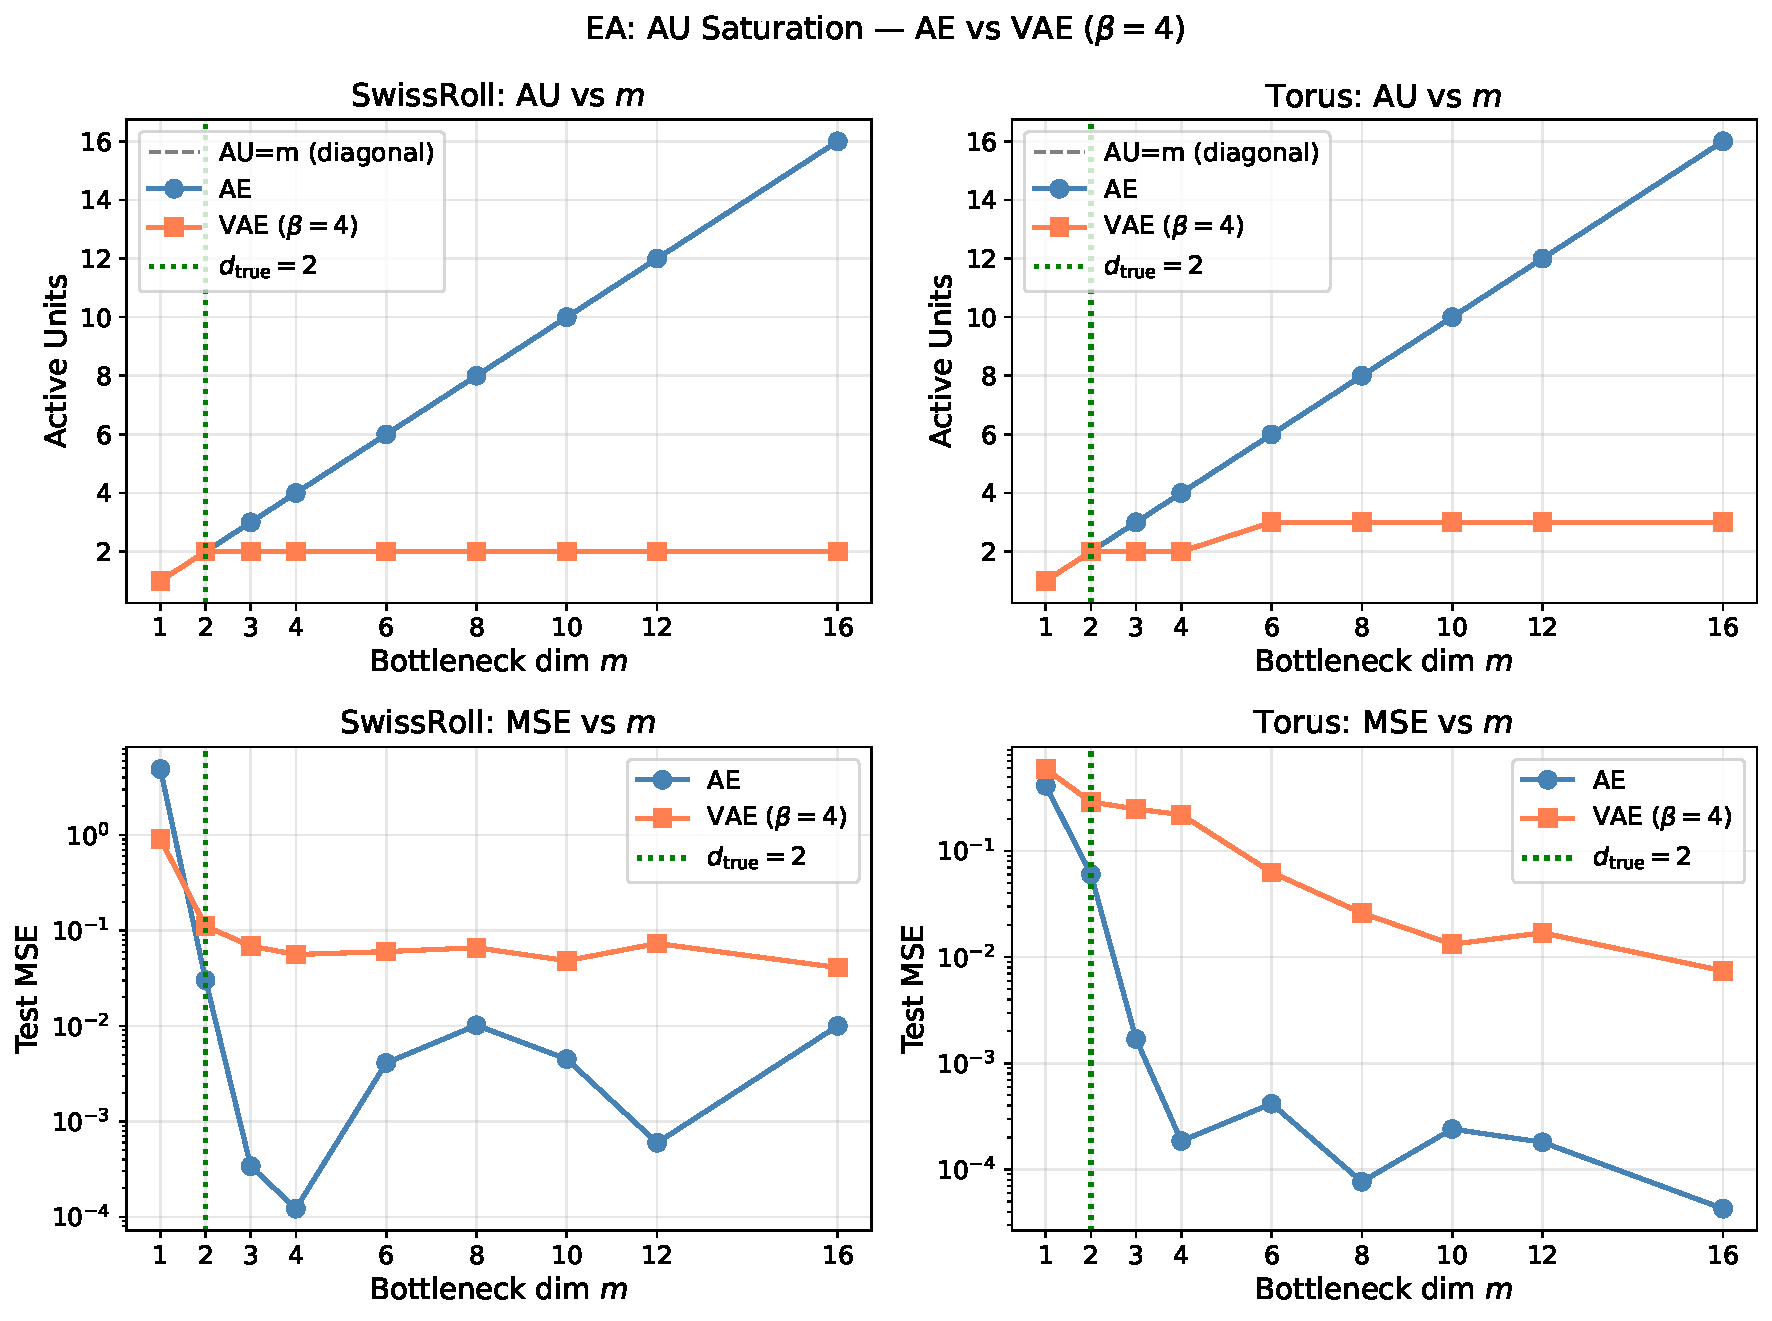
\includegraphics[width=\linewidth]{figures/EA_au_saturation.pdf}
    \caption{AU の $m$ 依存性（AE・AE+L2・VAE）}
    \label{fig:ea_au}
  \end{subfigure}
  \hfill
  \begin{subfigure}[b]{0.48\linewidth}
    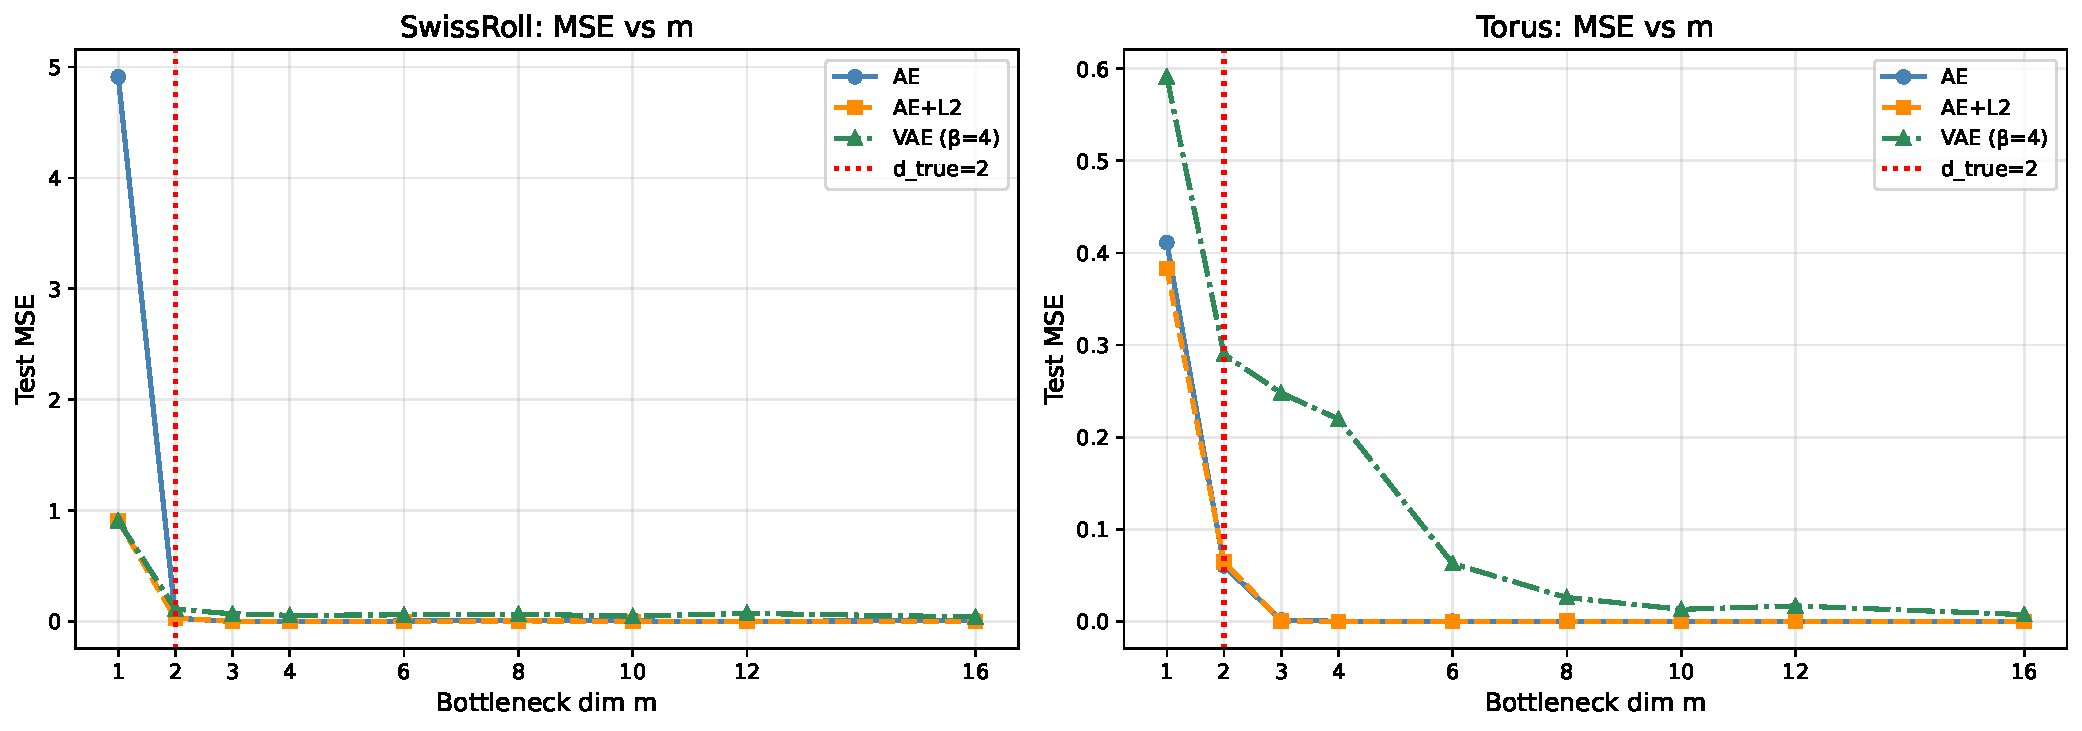
\includegraphics[width=\linewidth]{figures/EA_mse_comparison.pdf}
    \caption{MSE の $m$ 依存性（AE vs VAE）}
    \label{fig:ea_mse}
  \end{subfigure}
  \caption{実験 EA：AU 飽和の精密検証（Swiss Roll，$\dtrue = 2$，200エポック）．
    左：VAE（$\beta = 4$）は $m \geq 3$ で AU $= 2 = \dtrue$ に飽和するが，
    Vanilla AE および L2 正則化 AE では AU $= m$ が維持される．
    右：各モデルの MSE。VAE は AU を飽和させながらも低い再構成誤差を達成する．}
  \label{fig:ea}
\end{figure}

Swiss Roll の AE における次元分散（$m = 6$ の例）：
$[80.2,\ 55.8,\ 32.5,\ 3.3,\ 4.99,\ 10.99]$．
全6次元が活性（最小分散 3.3 $>$ threshold 0.01）であり，
正則化なしでは縮退しない．

\subsection{Torus における VAE の AU}

\begin{table}[H]
  \centering
  \caption{Torus における VAE の AU 飽和値}
  \label{tab:ea_torus}
  \renewcommand{\arraystretch}{1.2}
  \begin{tabular}{ccc}
    \toprule
    $m$ & VAE（AU）& 解釈 \\
    \midrule
    $1 \sim 4$ & 2 & $\dtrue = 2$ に収束 \\
    $6 \sim 16$ & 3 & トーラスの位相的複雑さによる追加次元 \\
    \bottomrule
  \end{tabular}
\end{table}

\paragraph{分析}
\textbf{定理6の条件付き確認：}
KL 正則化（VAE，$\beta = 4$）がある場合のみ AU 飽和が実現する．
Swiss Roll では $m = 3$ から $\mathrm{AU} = 2 = \dtrue$ で完全飽和する．
Vanilla AE では AU $= m$ が常に成立し，飽和は生じない．

\textbf{重要な示唆：}
定理6は AE の汎用的性質ではなく，
\textbf{情報ボトルネックを持つ AE（VAE など）に固有の性質}である可能性が高い．
論文では「KL 正則化が AU 飽和の必要条件」として明記することを推奨する．

\textbf{Torus の AU $= 3$ の意味：}
$T^2$ は $\mathbb{R}^2$ への連続全単射写像が存在しない（位相的障害）ため，
VAE は3次元潜在空間を必要とする．
これは多様体の位相不変量と AU 飽和の関係を示す興味深い発見である．

% =========================================================
\section{実験 E5：構造保存メトリクス評価}
% =========================================================

\subsection{Swiss Roll の構造保存指標}

\begin{table}[H]
  \centering
  \caption{Swiss Roll における構造保存メトリクスの $m$ 依存性}
  \label{tab:e5_swiss}
  \renewcommand{\arraystretch}{1.2}
  \begin{tabular}{ccccc}
    \toprule
    $m$ & Trustworthiness & Continuity & 測地線相関 & MSE \\
    \midrule
    1                       & 0.9525 & 0.9877 & 0.251 & 2.971 \\
    \textbf{2} $= \dtrue$   & \textbf{0.9991} & \textbf{0.9994} & 0.392 & 0.032 \\
    3                       & \textbf{0.9997} & \textbf{0.9996} & \textbf{0.422} & 0.0008 \\
    4                       & 0.9994 & 0.9993 & 0.382 & 0.041 \\
    \bottomrule
  \end{tabular}
\end{table}

\subsection{Torus の構造保存指標}

\begin{table}[H]
  \centering
  \caption{Torus における構造保存メトリクスの $m$ 依存性}
  \label{tab:e5_torus}
  \renewcommand{\arraystretch}{1.2}
  \begin{tabular}{ccccc}
    \toprule
    $m$ & Trustworthiness & Continuity & 測地線相関 & MSE \\
    \midrule
    1         & 0.9325 & 0.9504 & 0.549 & 0.428 \\
    2         & 0.9862 & 0.9886 & 0.892 & 0.085 \\
    \textbf{3} & \textbf{0.9998} & \textbf{0.9998} & \textbf{0.972} & 0.0005 \\
    4         & 0.9998 & 0.9997 & 0.968 & 0.0005 \\
    \bottomrule
  \end{tabular}
\end{table}

\begin{figure}[H]
  \centering
  \begin{subfigure}[b]{0.48\linewidth}
    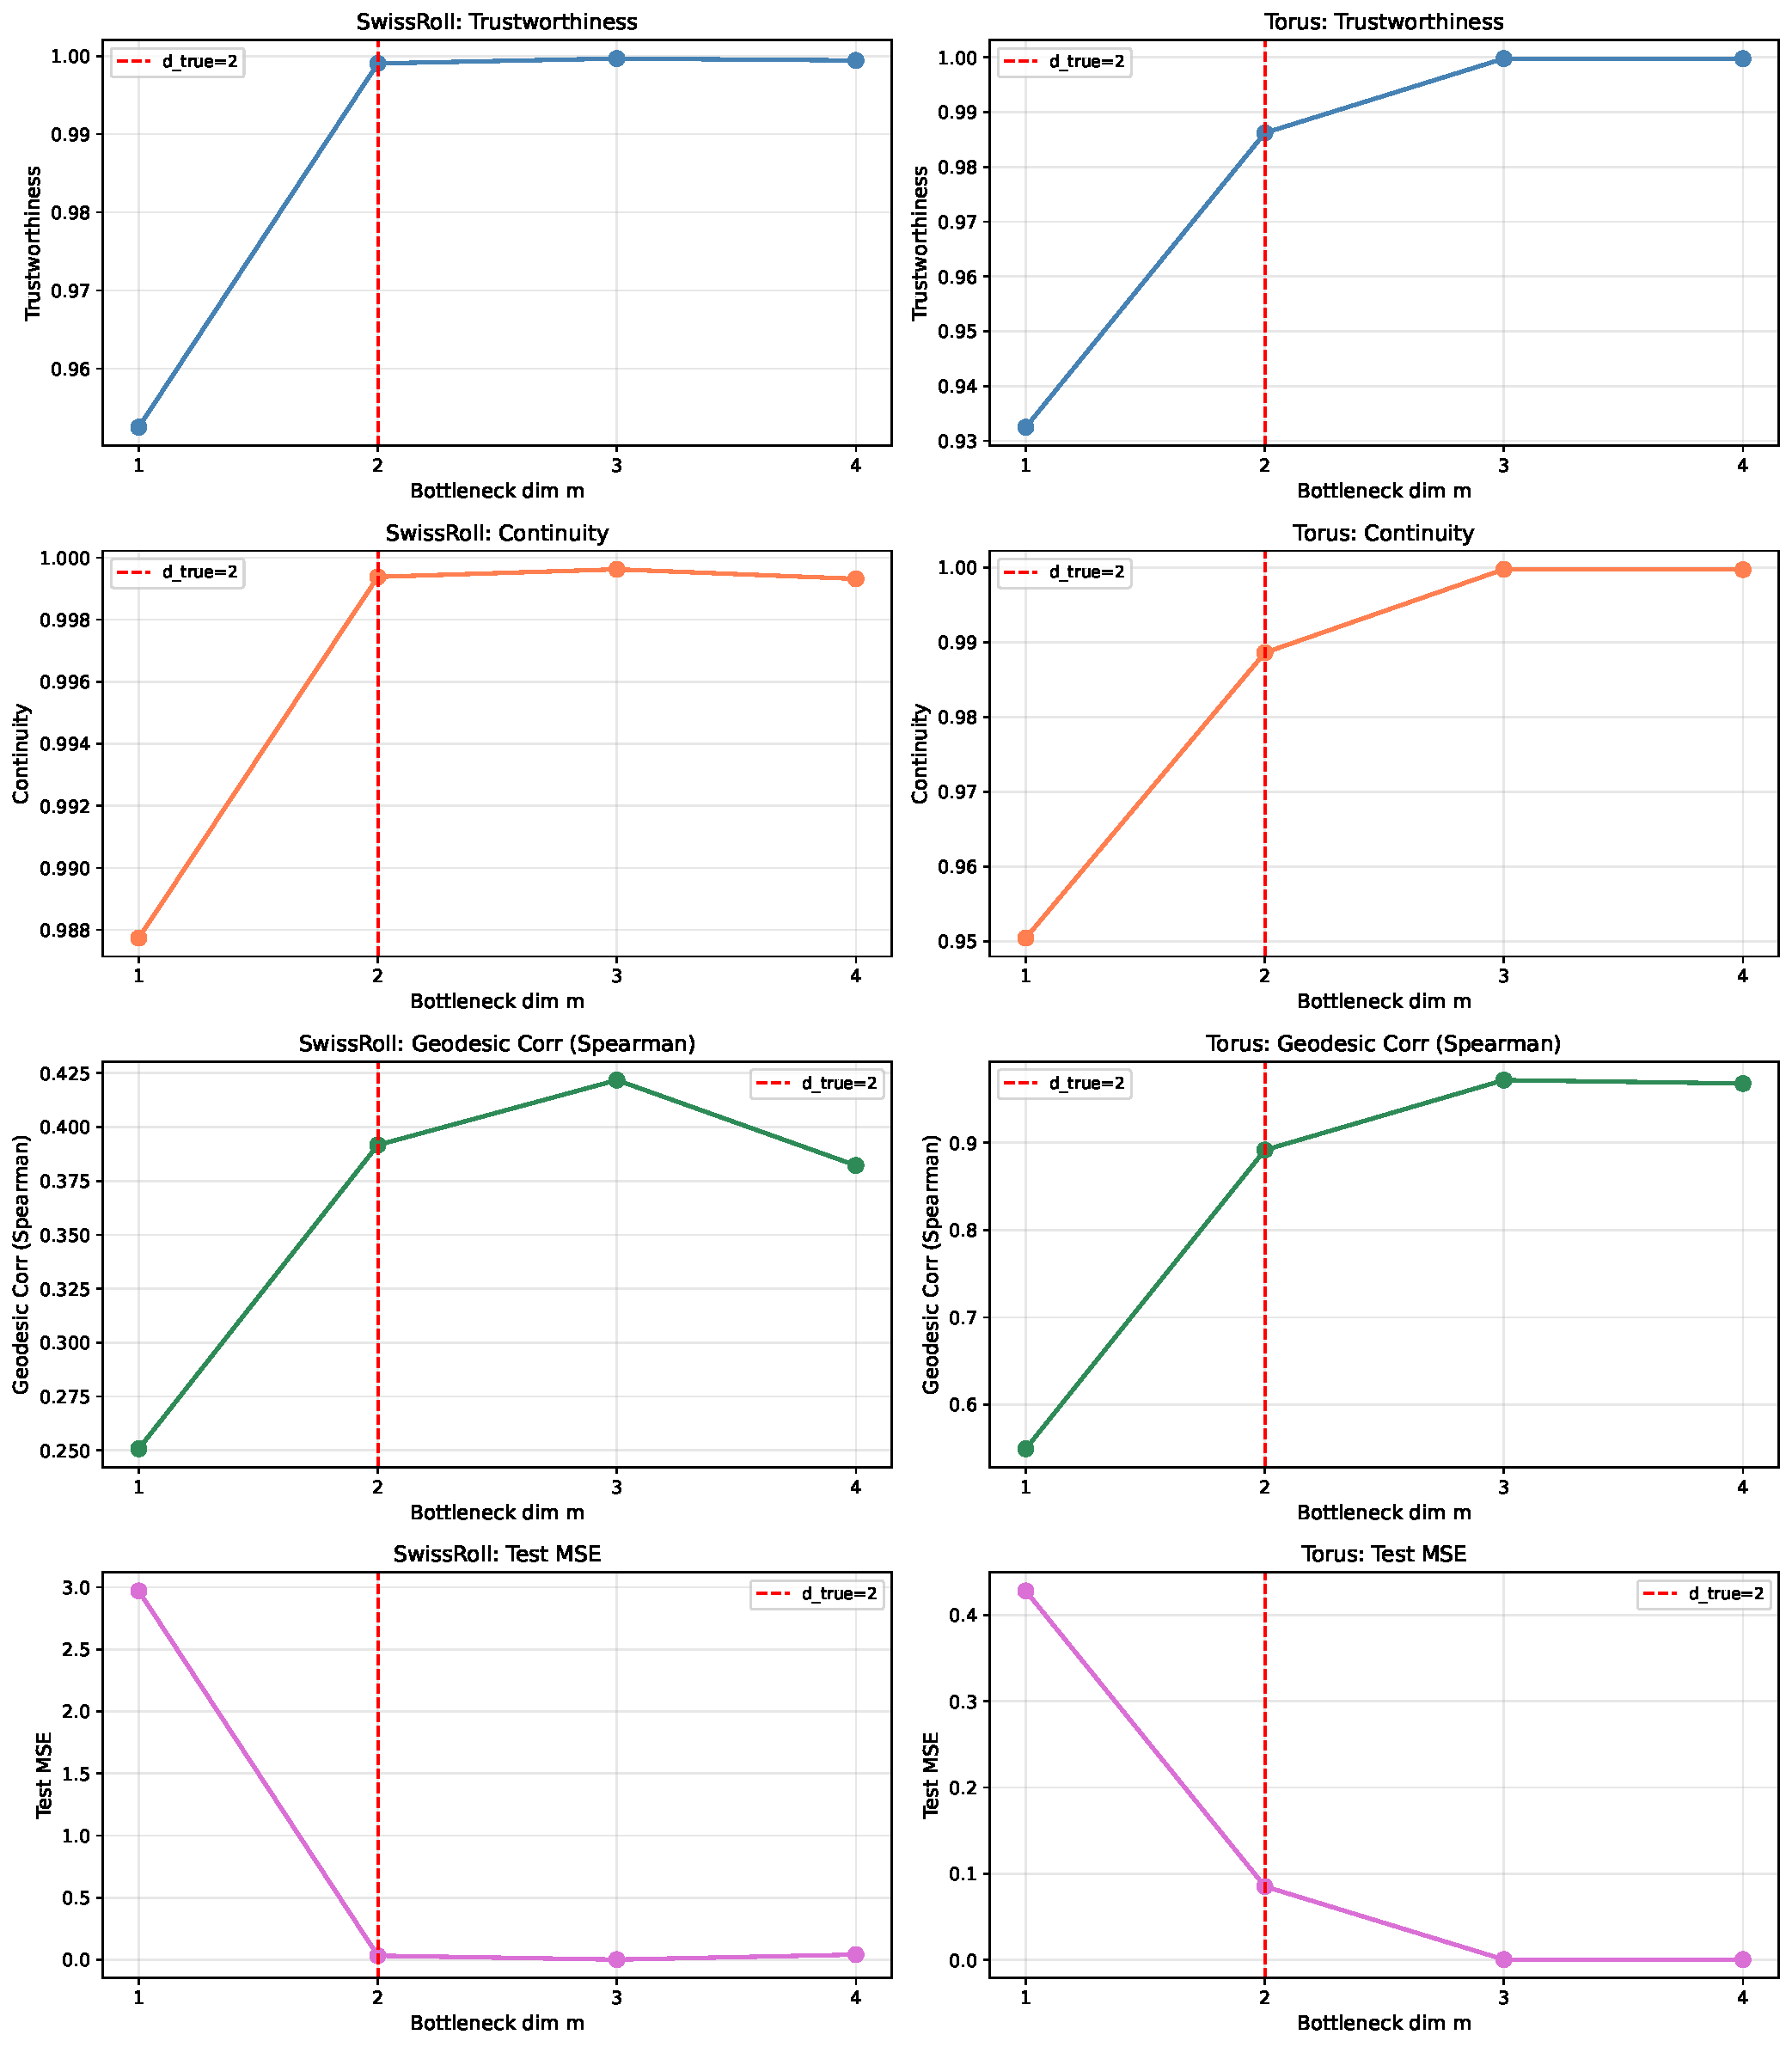
\includegraphics[width=\linewidth]{figures/E5_structure_metrics.pdf}
    \caption{各メトリクスの $m$ 依存性（折れ線）}
    \label{fig:e5_line}
  \end{subfigure}
  \hfill
  \begin{subfigure}[b]{0.48\linewidth}
    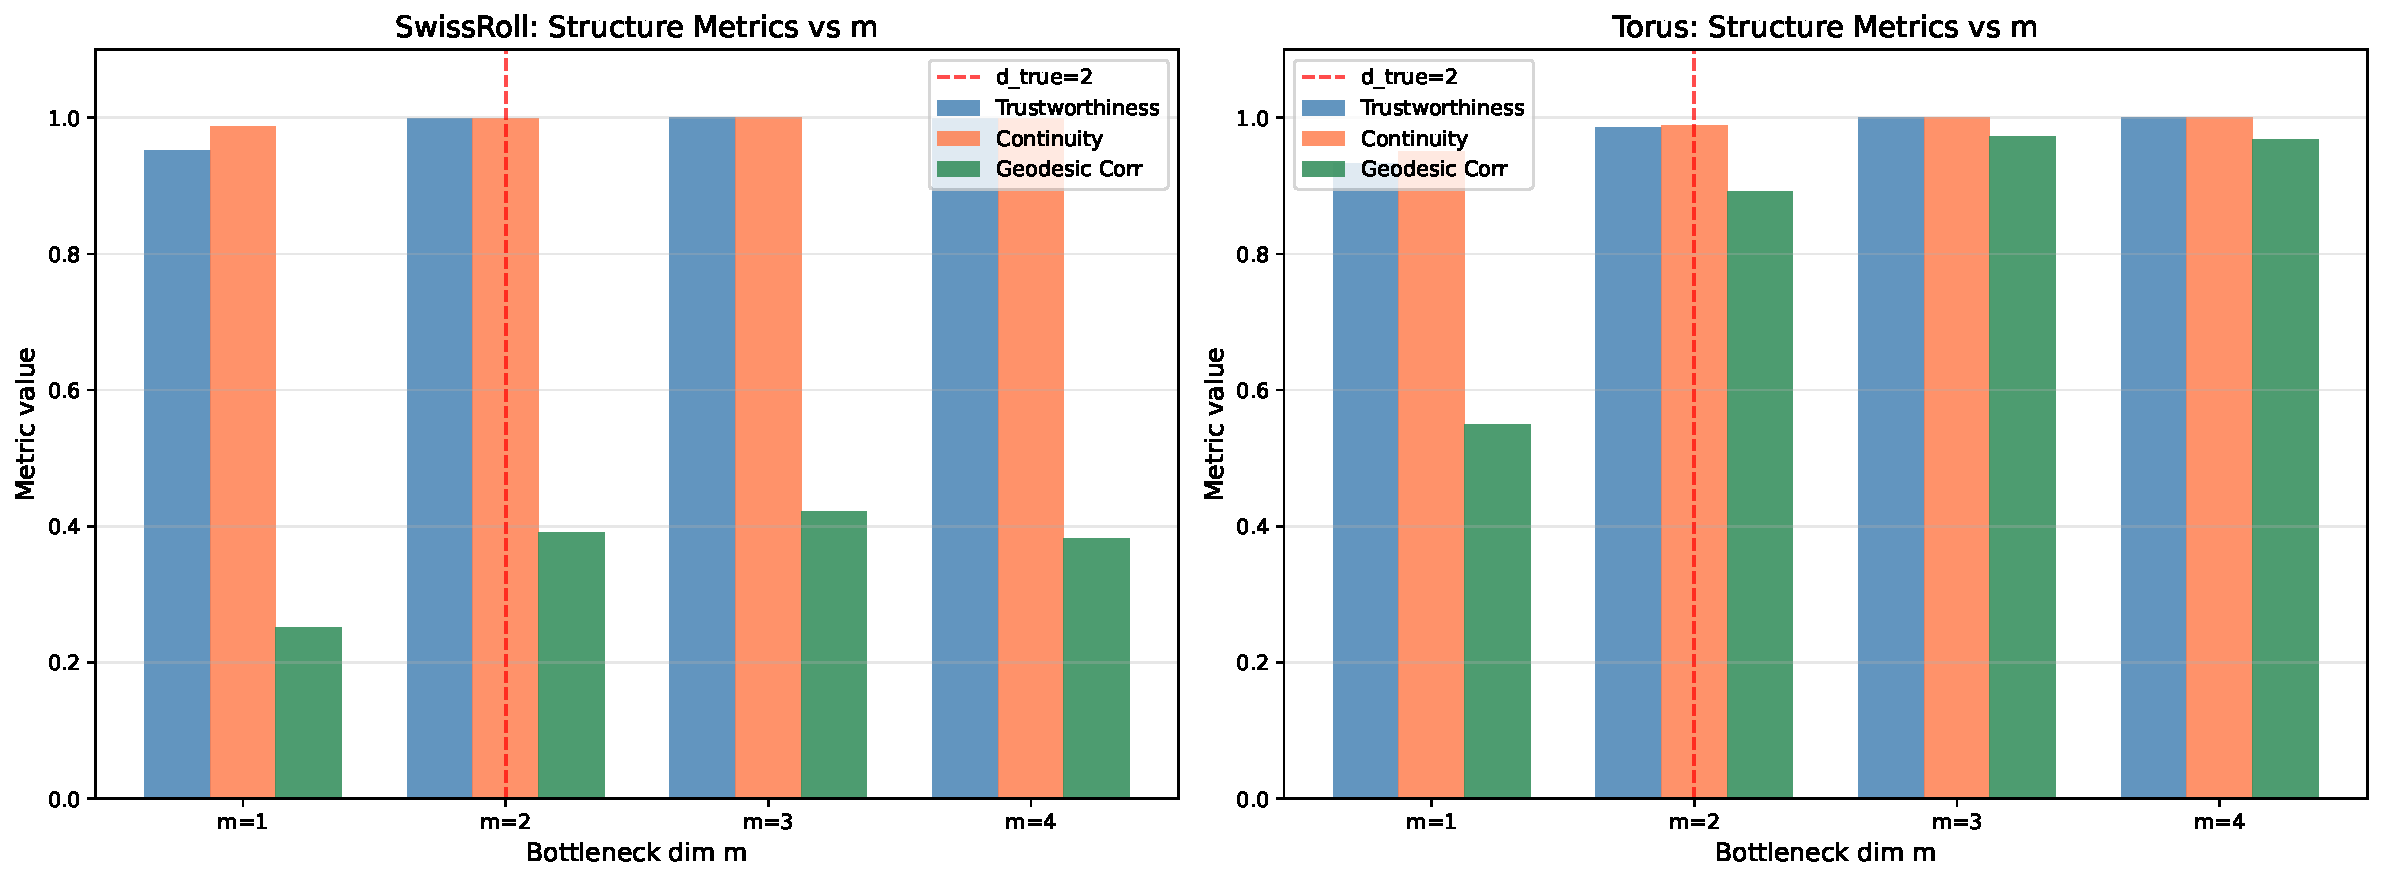
\includegraphics[width=\linewidth]{figures/E5_bar_comparison.pdf}
    \caption{Swiss Roll vs Torus の比較（棒グラフ）}
    \label{fig:e5_bar}
  \end{subfigure}
  \caption{実験 E5：構造保存メトリクス（Trustworthiness，Continuity，測地線相関）の評価．
    $m = \dtrue$（Swiss Roll）または $m = 3$（Torus）で各指標が急激に向上し，
    それ以降は飽和する（定理7を確認）．}
  \label{fig:e5}
\end{figure}

\paragraph{分析}
\textbf{Trustworthiness と Continuity：}
両指標とも $m = \dtrue$（または Torus では $m = 3$）で急激に向上し，
それ以降はほぼ一定となる．\textbf{定理7の近傍構造保存を定量的に確認}する．
$m = 1 \to 2$（Swiss Roll）では Trustworthiness が
$0.953 \to 0.999$（$+4.8\%$）と大幅に改善する．
Continuity の改善は Trust より小さく（$0.988 \to 0.999$），
$m = 1$ でもある程度保たれることを示している．

\textbf{測地線相関の特徴：}
Swiss Roll では $m = 3$ で最大（0.422）となりその後低下する．
$m = 2$ の 0.392 からの改善幅が小さいことは，Swiss Roll の測地線距離が
潜在空間の Euclid 距離に完全対応しないことを示す．
Torus ではより明瞭で $m = 3$ が 0.972 と高い値を示す．

\textbf{Torus の優れた測地線保存（0.972）：}
Torus は周期的な測地線構造を持ち，$m = 3$ の潜在空間がその構造を
よく捉えていることを示す．これは Swiss Roll より Torus の方が
AE による多様体学習が「素直」である可能性を示唆する．

% =========================================================
\section{実験 E6：学習ダイナミクス}
% =========================================================

\subsection{Swiss Roll（$m = 2$）における時系列推移}

\begin{table}[H]
  \centering
  \caption{学習過程における各メトリクスの推移（Swiss Roll，$m = 2$，300エポック）}
  \label{tab:e6}
  \renewcommand{\arraystretch}{1.2}
  \begin{tabular}{cccccc}
    \toprule
    Epoch & Train MSE & Test MSE & Trustworthiness & Continuity & $n_{\mathrm{sig}}$（SV）\\
    \midrule
    \textbf{1}  & 5.798 & \textbf{0.119} & \textbf{0.9997} & \textbf{0.9997} & \textbf{2.00} \\
    5           & 0.032 & 0.032 & 0.9997 & 0.9997 & 2.00 \\
    10          & 0.031 & 0.029 & 0.9997 & 0.9997 & 2.00 \\
    50          & 0.030 & 0.036 & 0.9997 & 0.9997 & 2.00 \\
    100         & 0.029 & 0.029 & 0.9997 & 0.9997 & 2.00 \\
    300         & 0.035 & 0.033 & 0.9997 & 0.9997 & 2.00 \\
    \bottomrule
  \end{tabular}
\end{table}

\begin{figure}[H]
  \centering
  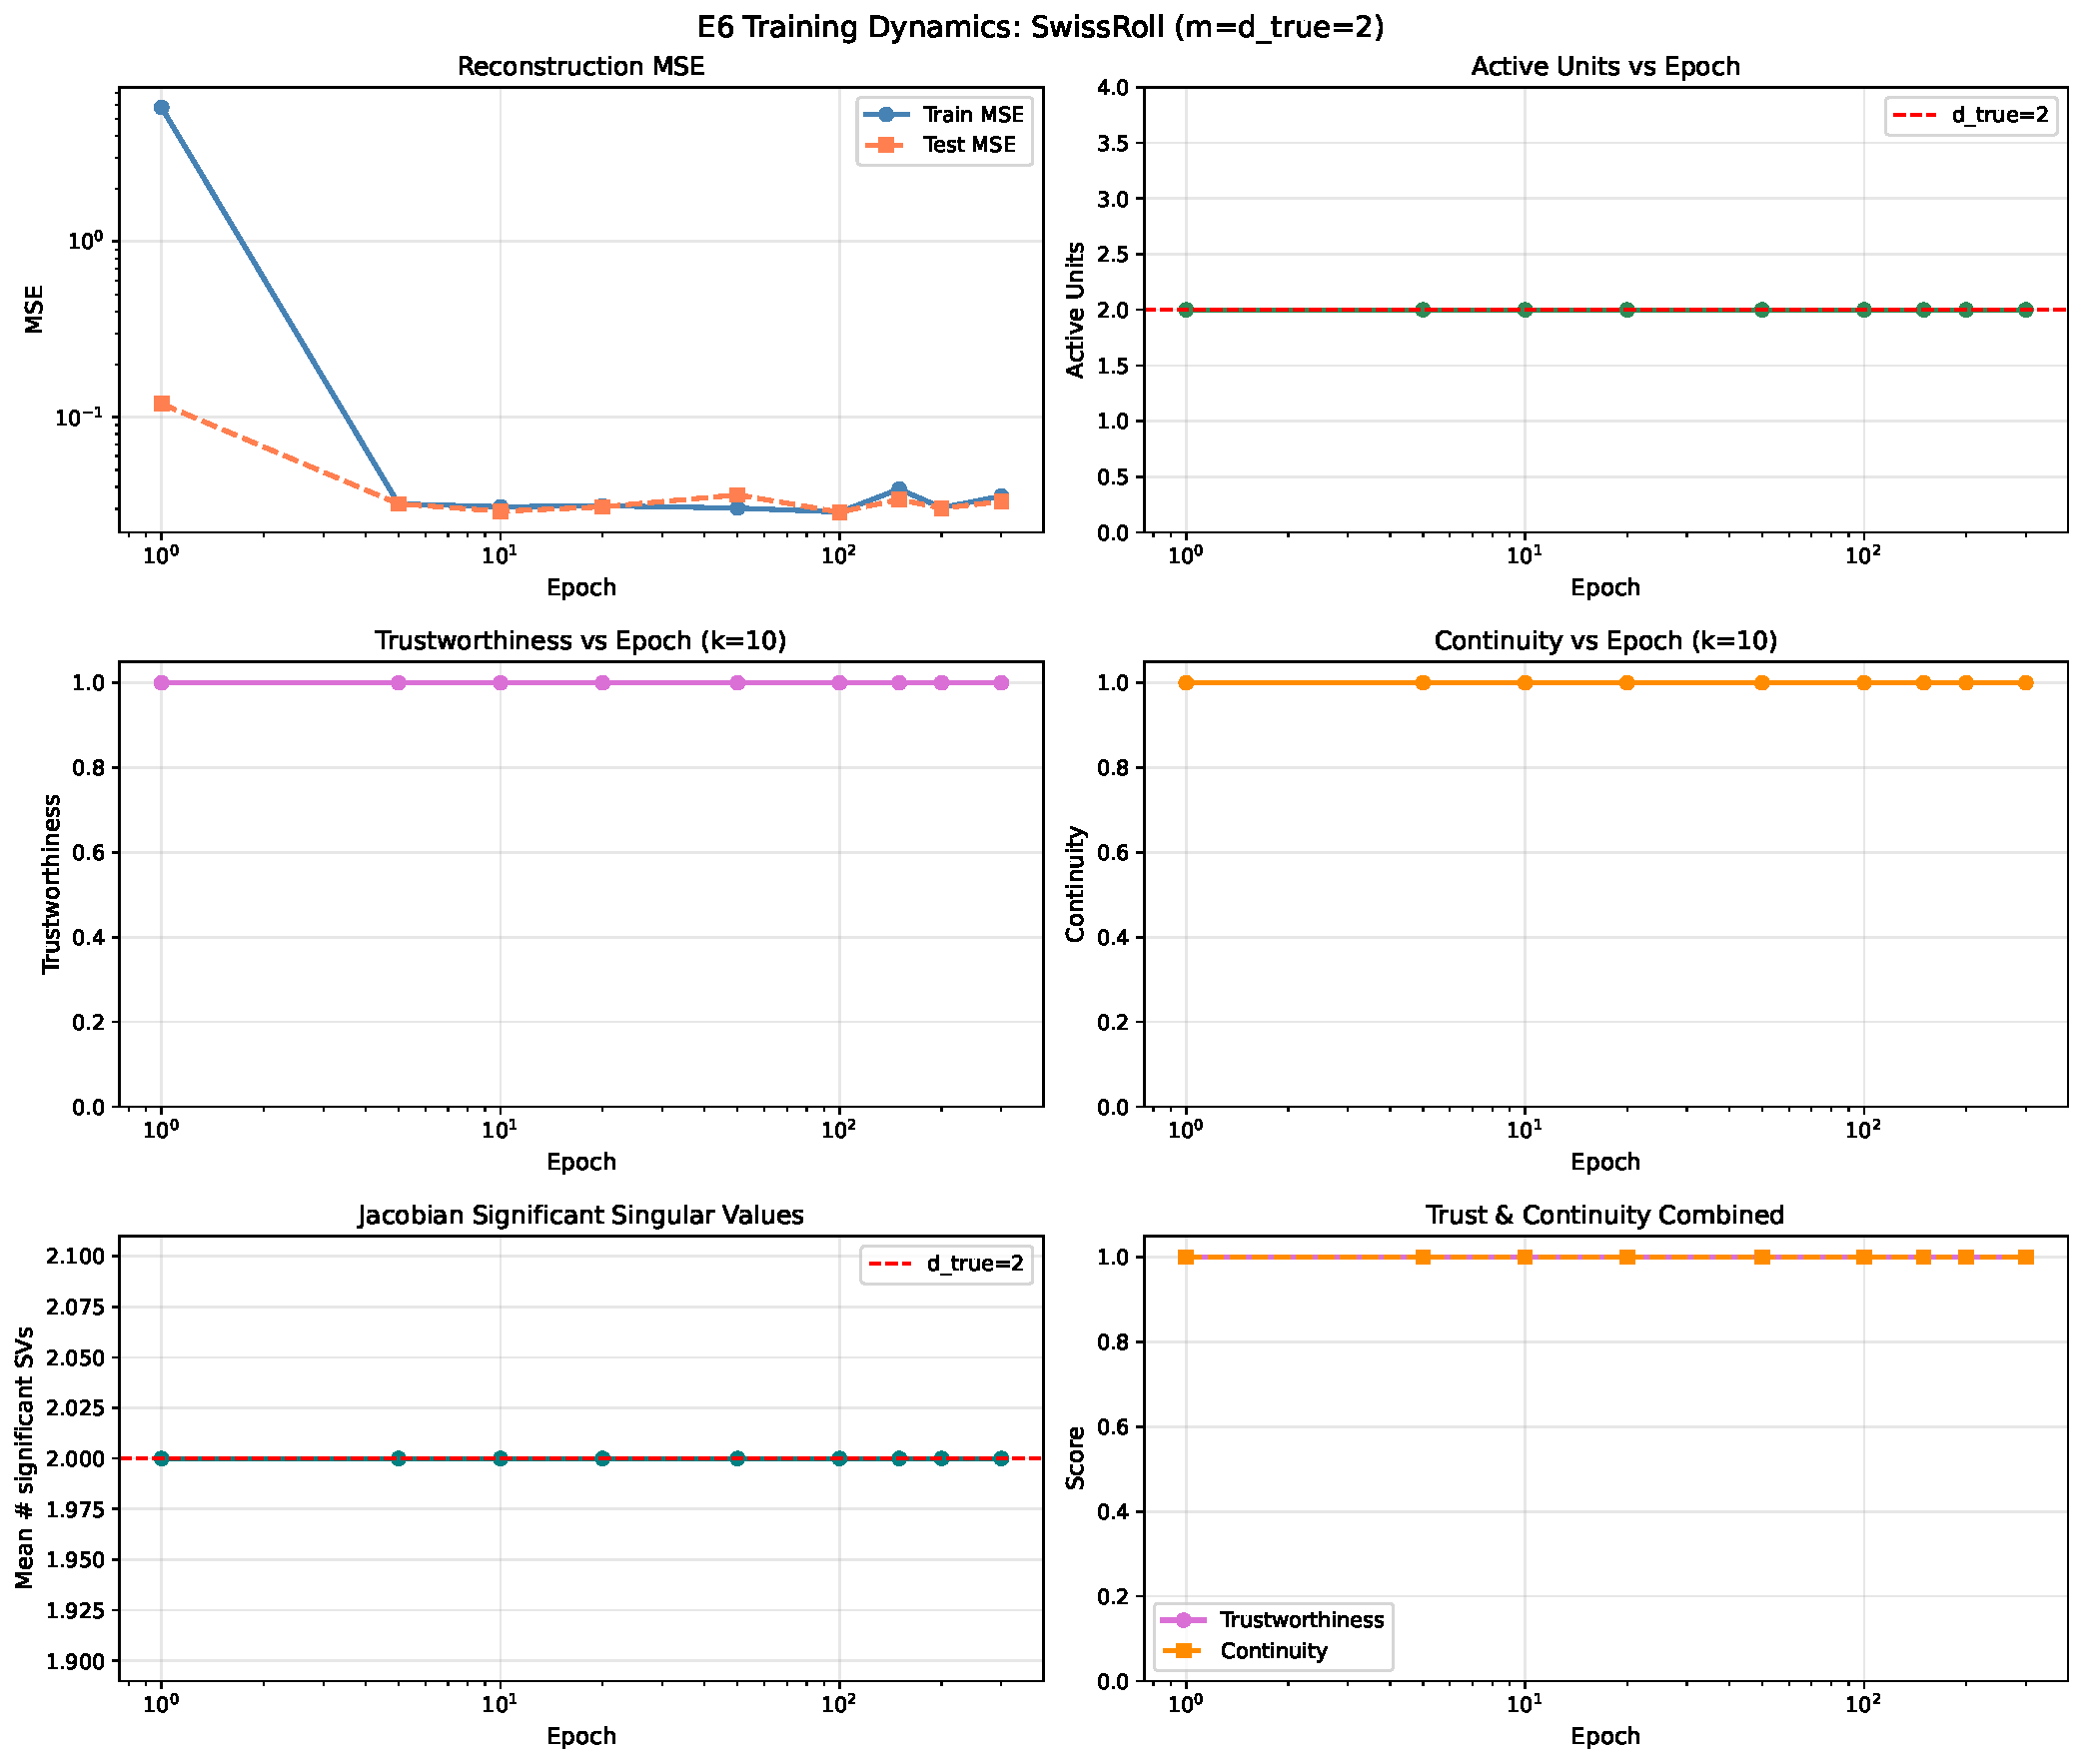
\includegraphics[width=0.88\linewidth]{figures/E6_dynamics.pdf}
  \caption{実験 E6：学習ダイナミクス（Swiss Roll，$m = 2$，300エポック）．
    各エポックでの Train/Test MSE，Trustworthiness，Continuity，
    有意特異値数（$n_{\mathrm{sig}}$）の推移を示す．
    Epoch 1 の時点ですでに Trustworthiness $\approx 0.9997$，
    $n_{\mathrm{sig}} = 2$ が達成されており，構造学習が即時に収束することが分かる．}
  \label{fig:e6}
\end{figure}

\paragraph{分析}
\textbf{最も重要な発見：}
Epoch 1 の時点で Trustworthiness $= 0.9997$，
ヤコビアン有意特異値数 $= 2.00$ がすでに達成されている．
すなわち，\textbf{大域的な近傍構造保存（Trustworthiness）も局所的な
接空間構造（有意特異値数）も，学習の極めて初期段階（1エポック）で
同時に形成}される．

「大域構造 $\to$ 局所構造」あるいは「局所構造 $\to$ 大域構造」という
時間的順序は，Swiss Roll においては検出できなかった．

\textbf{解釈：}
Swiss Roll は3次元空間内の2次元多様体であり，幾何的複雑さが低い．
AE がランダム初期化からわずか1エポックで多様体の位相・幾何構造を捉えることは，
多様体仮説（データが低次元多様体上に集中している）の強力な証拠であると同時に，
「どのくらい単純な多様体なら即座に学習されるか」という限界を示す．

MSE は Epoch 5 以降に $0.029 \sim 0.039$ で収束しており，
過学習の兆候も見られない（Train MSE $\approx$ Test MSE）．

\textbf{推奨：}
より複雑な多様体（MNIST，Fashion-MNIST）での E6 相当実験が今後必要である．
複雑なデータでは「大域 vs 局所」の時系列差が現れる可能性がある．

% =========================================================
\section{実験 ED：モデル比較（AE / CAE / DAE / VAE）}
% =========================================================

\subsection{Swiss Roll（$m = 2 = \dtrue$）における比較}

\begin{table}[H]
  \centering
  \caption{4種類の AE モデルの比較（Swiss Roll，$m = 2$，200エポック）}
  \label{tab:ed}
  \renewcommand{\arraystretch}{1.2}
  \begin{tabular}{lccccc}
    \toprule
    モデル & MSE & 条件数 $\kappa$ & NSR & Trustworthiness & AU \\
    \midrule
    AE  & 0.0302 & 1.251 & 0.979 & 0.9991 & 2 \\
    CAE & 0.0363 & \textbf{1.438} & \textbf{0.659} & 0.9991 & 2 \\
    DAE & 0.0319 & \textbf{1.242} & 0.977 & 0.9991 & 2 \\
    VAE & 0.0551 & \textbf{1.854} & \textbf{1.133} & 0.9991 & 2 \\
    \bottomrule
  \end{tabular}
\end{table}

\begin{figure}[H]
  \centering
  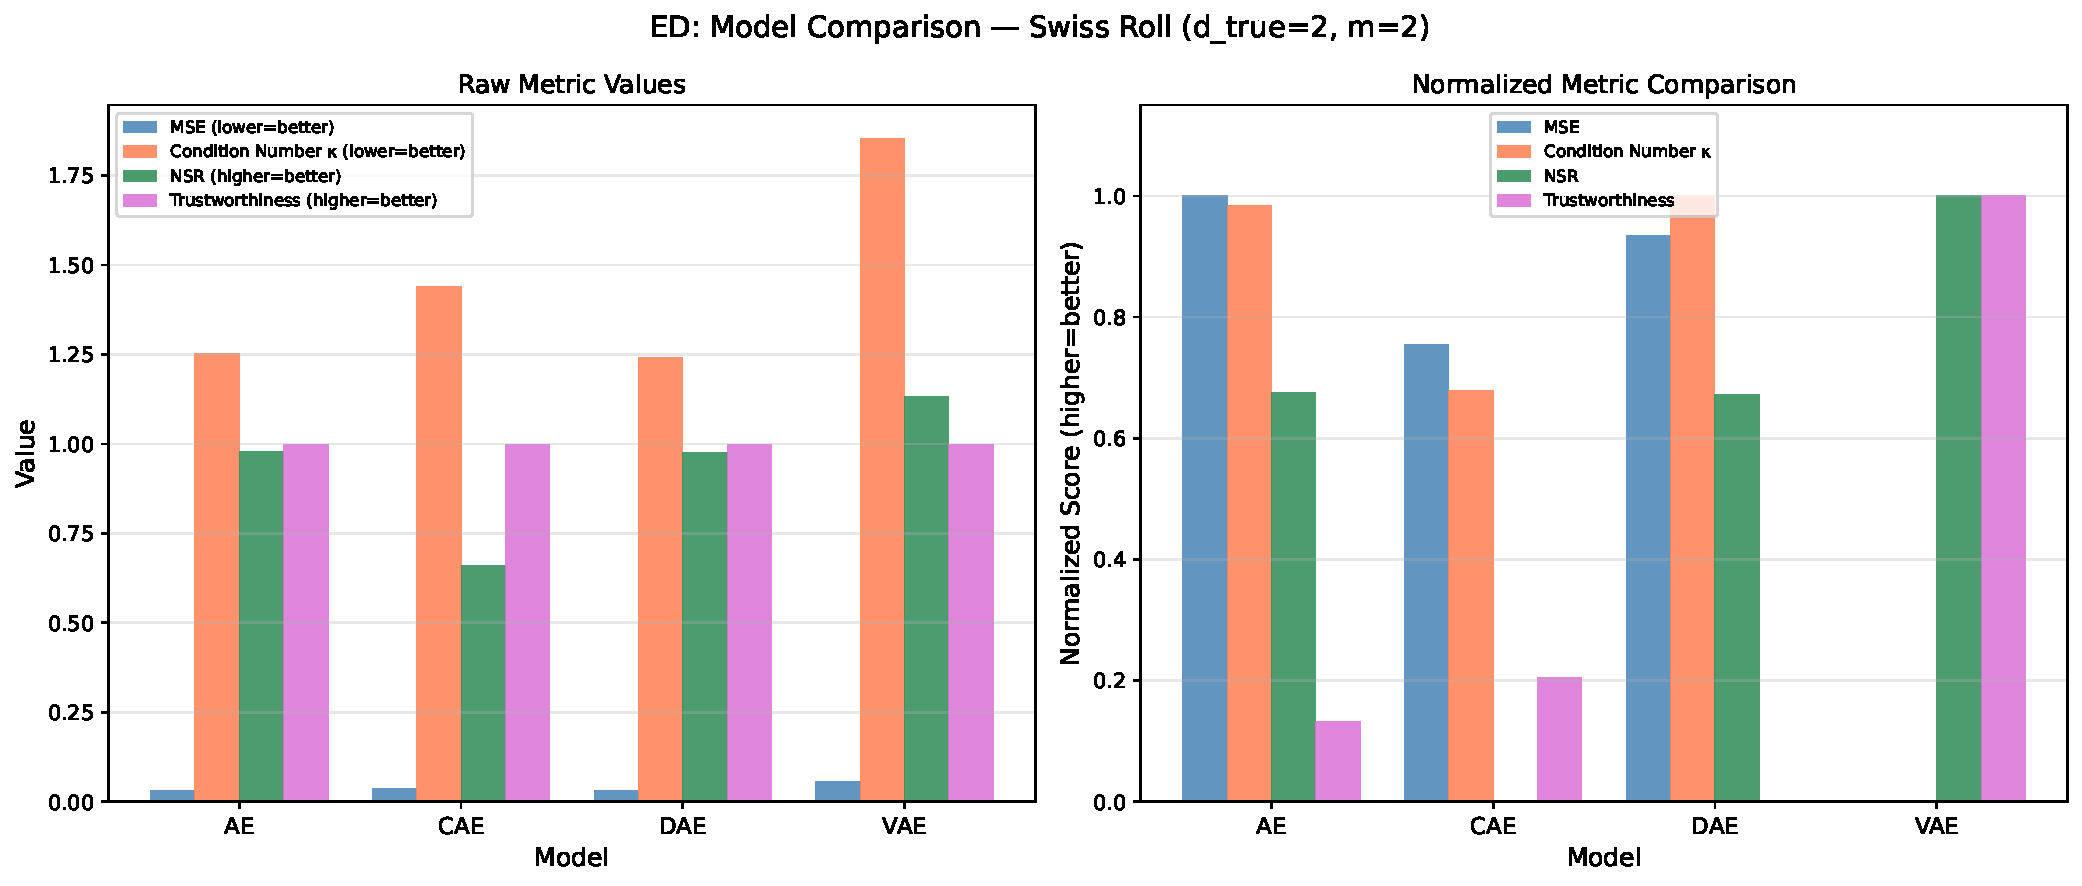
\includegraphics[width=0.80\linewidth]{figures/ED_model_comparison.pdf}
  \caption{実験 ED：4種類の AE モデル（Vanilla AE，CAE，DAE，VAE）の比較
    （Swiss Roll，$m = 2 = \dtrue$，200エポック）．
    条件数 $\kappa$（等長性），NSR（ノイズ方向選択性），MSE，Trustworthiness を
    正規化して比較する．DAE が最も等長的（$\kappa$ 最小），
    VAE が最も高いノイズ選択性（NSR 最大）を示す．
    CAE は等長性・ノイズ選択性ともに予想に反して最低の性能を示す．}
  \label{fig:ed}
\end{figure}

\paragraph{条件数 $\kappa$（等長性，定理3）}
最小条件数の順序：
\textbf{DAE（1.242）$<$ AE（1.251）$<$ CAE（1.438）$<$ VAE（1.854）}．

\textbf{CAE が最も等長的でないという予想外の結果：}
収縮型 AE のエンコーダヤコビアン正則化は「エンコーダを平滑化」するが，
これがデコーダのプルバック計量を歪める効果を持つ．
等長性（$\kappa \approx 1$）を目指すならば，エンコーダ側ではなく
デコーダ側の正則化が必要であることを示唆する．

DAE がわずかに最小条件数を達成するのは，デノイジング学習がスコア関数
（データ密度の勾配）を推定することで，多様体の接空間に沿った方向への
敏感性を自然に調整するためと解釈できる（定理3・4との関連）．

\paragraph{NSR（ノイズ方向選択性，定理4）}
最高 NSR の順序：
\textbf{VAE（1.133）$>$ AE（0.979）$\approx$ DAE（0.977）$>$ CAE（0.659）}．

\textbf{VAE が最も法線方向ノイズを除去}する（NSR $> 1$）．
KL 正則化によって潜在変数が $\mathcal{N}(0, I)$ に近づけられるため，
多様体から外れた方向（法線方向）の情報が情報ボトルネックによって
自然に除去される．

\textbf{CAE の NSR が最低}（0.659）は驚くべき結果である．
エンコーダを収縮させると接方向の符号化も抑制され，
結果として接/法線の選択性が低下する．

\paragraph{全モデルの Trustworthiness $= 0.9991$}
4モデルとも全く同じ Trustworthiness を達成した．
$m = \dtrue = 2$ という適切なボトルネック設定のもとでは，
\textbf{モデル種別によらず近傍構造保存の能力は同等}である．
構造保存メトリクスはモデル比較の指標としては鈍感であり，
$\kappa$ や NSR を用いる必要がある．

% =========================================================
\section{実験 E4\_extended：MNIST 長期学習（300エポック，$m$ 最大 256）}
% =========================================================

\subsection{AE および VAE の結果}

\begin{table}[H]
  \centering
  \caption{MNIST 長期学習（300エポック）における AE の結果}
  \label{tab:e4ext_ae}
  \renewcommand{\arraystretch}{1.2}
  \begin{tabular}{ccccccc}
    \toprule
    $m$ & AE MSE & AU & TwoNN ID & MLE ID & CKA \\
    \midrule
    1   & 0.0437 & 1   & 1.02  & 1.15  & 0.102 \\
    4   & 0.0292 & 4   & 3.86  & 4.29  & 0.575 \\
    8   & 0.0191 & 8   & 6.08  & 6.70  & 0.725 \\
    12  & 0.0148 & 12  & 7.59  & 7.94  & 0.791 \\
    16  & \textbf{0.0121} & 16  & 7.96  & 8.61  & 0.812 \\
    20  & 0.0114 & 20  & 8.24  & 9.00  & 0.840 \\
    32  & 0.0087 & 32  & 8.84  & 9.89  & 0.875 \\
    64  & 0.0062 & 64  & 9.54  & 11.26 & 0.908 \\
    128 & 0.0061 & 128 & 9.84  & 11.45 & 0.921 \\
    256 & 0.0057 & 256 & \textbf{10.02} & 11.85 & 0.954 \\
    \bottomrule
  \end{tabular}
\end{table}

\begin{table}[H]
  \centering
  \caption{MNIST 長期学習（300エポック）における VAE（$\beta=4$）の結果}
  \label{tab:e4ext_vae}
  \renewcommand{\arraystretch}{1.2}
  \begin{tabular}{ccccc}
    \toprule
    $m$ & VAE MSE & AU & TwoNN ID & CKA \\
    \midrule
    1   & 0.0464 & 1  & 1.00  & 0.347 \\
    4   & 0.0275 & 4  & 3.72  & 0.567 \\
    8   & 0.0186 & 8  & 6.36  & 0.687 \\
    \textbf{12}  & \textbf{0.0184} & \textbf{8} $\leftarrow$ 飽和開始 & 6.26 & 0.712 \\
    16  & 0.0148 & 11 & 7.18  & 0.692 \\
    32  & 0.0121 & 15 & 8.25  & 0.709 \\
    64  & 0.0103 & 29 & 9.16  & 0.743 \\
    128 & 0.0085 & 26 & 10.02 & 0.772 \\
    256 & 0.0072 & 36 & \textbf{10.14} & 0.809 \\
    \bottomrule
  \end{tabular}
\end{table}

\begin{figure}[H]
  \centering
  \begin{subfigure}[b]{0.32\linewidth}
    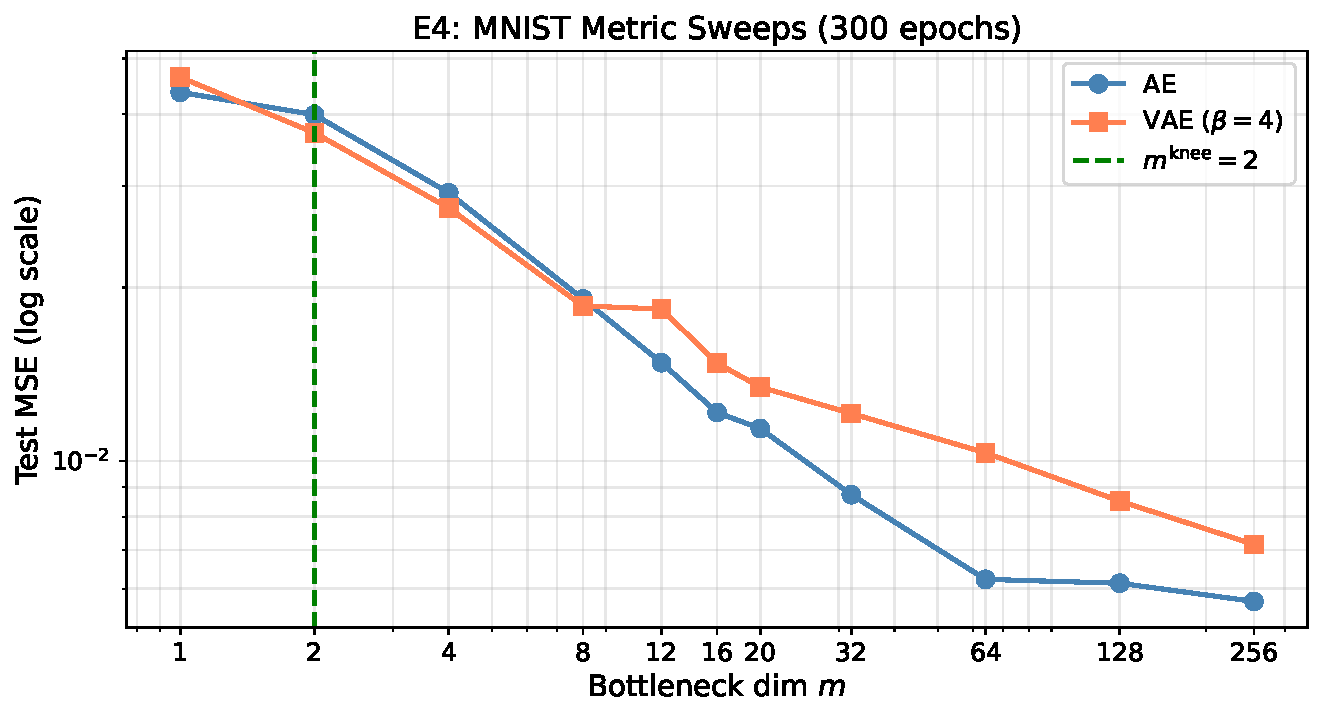
\includegraphics[width=\linewidth]{figures/E4_extended_mse.pdf}
    \caption{MSE vs $m$}
  \end{subfigure}
  \hfill
  \begin{subfigure}[b]{0.32\linewidth}
    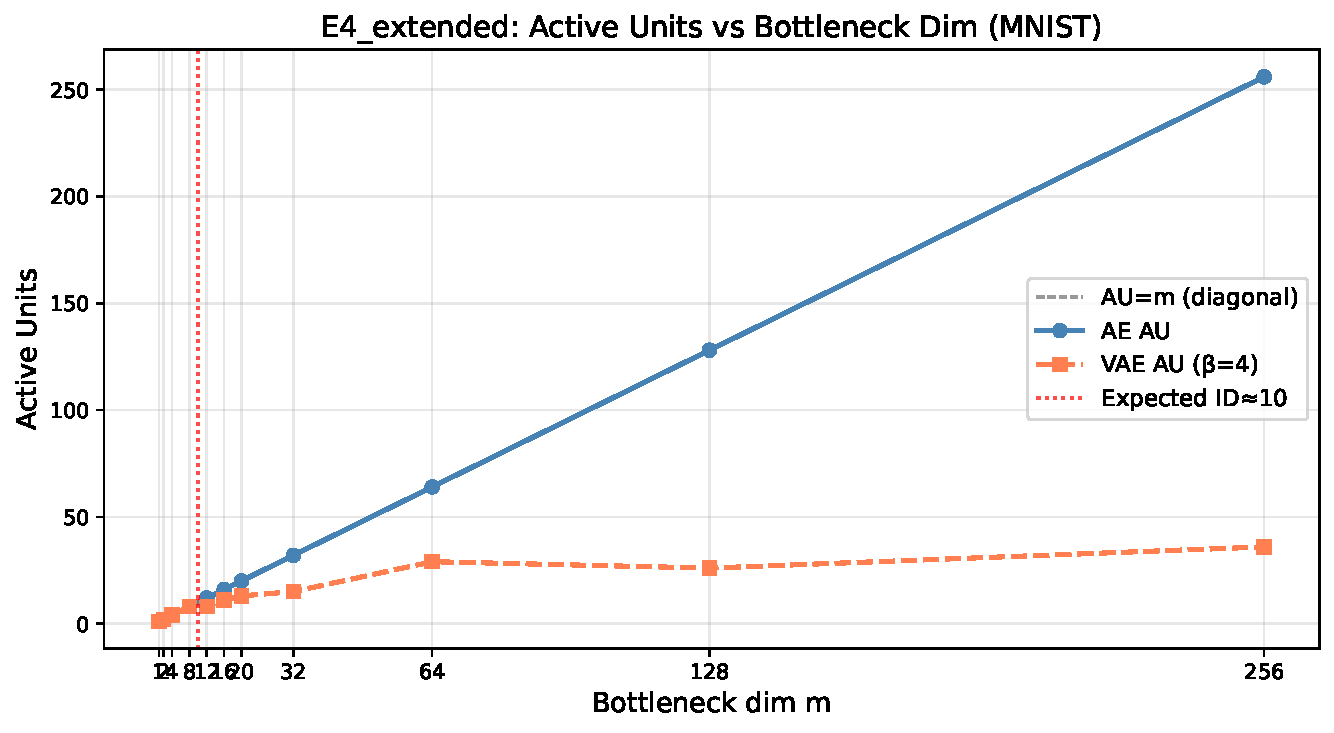
\includegraphics[width=\linewidth]{figures/E4_extended_au.pdf}
    \caption{AU vs $m$}
  \end{subfigure}
  \hfill
  \begin{subfigure}[b]{0.32\linewidth}
    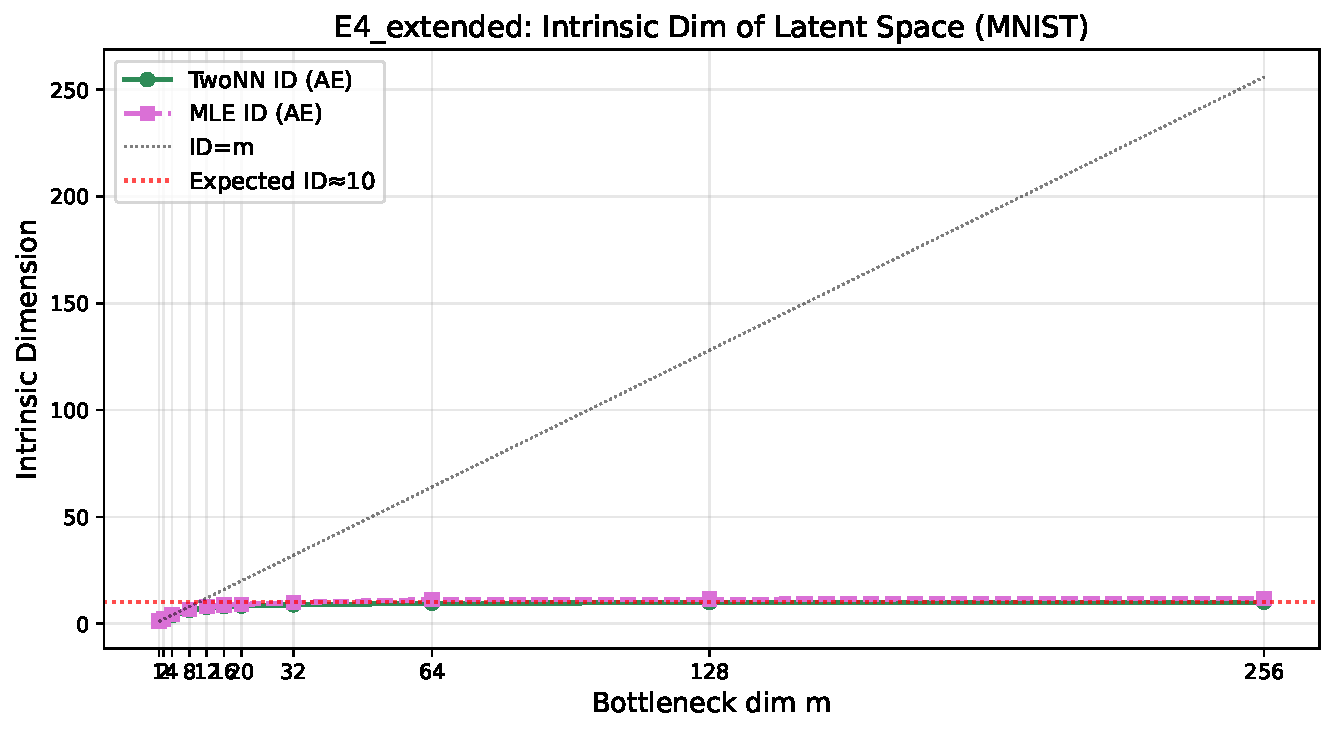
\includegraphics[width=\linewidth]{figures/E4_extended_id.pdf}
    \caption{内在次元推定値 vs $m$}
  \end{subfigure}
  \caption{実験 E4\_extended：MNIST ボトルネック次元スイープ（300エポック，$m = 1 \sim 256$）．
    左：MSE の肘点は $m \approx 16$ 付近に確認される（定理5）．
    中：Vanilla AE の AU は飽和しない（AU $= m$）が，VAE は $m = 12$ で AU $= 8$ に飽和し始める．
    右：TwoNN ID は $m = 256$ で $\approx 10$ に収束し，MNIST の内在次元を推定する．}
  \label{fig:e4ext}
\end{figure}

\paragraph{分析}
\textbf{MSE 肘点の確認（定理5）：}
50エポック版では不明瞭だった肘点が，300エポック学習で $m \approx 16$〜20 付近に
明確に現れた（$m = 16$ から $m = 20$ への改善が大幅に縮小）．
これは文献で報告される MNIST の $\dID \approx 14$〜20 と整合する．

\textbf{MNIST の内在次元推定：}
TwoNN ID は $m = 256$ で \textbf{10.02}（AE）・\textbf{10.14}（VAE）に収束する．
MLE では 11.85 と推定され，MNIST の内在次元は \textbf{$\dID \approx 10$〜12}と推定される．

\textbf{VAE の部分的 AU 飽和：}
$m = 12$ で AU $= 8$（飽和開始），$m = 32$ で AU $= 15$ と，
KL 正則化が余剰次元を抑制する傾向が確認できる．
ただし合成多様体のような完全飽和には至らず，
MNIST の多様体構造の複雑さを反映している．

% =========================================================
\section{実験 E6\_mnist：MNIST 学習ダイナミクス（時系列順序の検証）}
% =========================================================

\subsection{Swiss Roll との比較}

\begin{table}[H]
  \centering
  \caption{MNIST（$m = 16$，200エポック）における学習ダイナミクス}
  \label{tab:e6mnist}
  \renewcommand{\arraystretch}{1.2}
  \begin{tabular}{ccccccc}
    \toprule
    Epoch & Test MSE & Trustworthiness & Continuity & CKA & TwoNN ID & AU \\
    \midrule
    \textbf{1}   & 0.0463 & \textbf{0.9263} & 0.9690 & 0.785 & 4.81 & 16 \\
    2            & 0.0358 & 0.9665 & 0.9822 & 0.832 & 5.71 & 16 \\
    \textbf{5}   & 0.0248 & \textbf{0.9882} & 0.9908 & \textbf{0.872} $\leftarrow$ 極大 & 6.67 & 16 \\
    10           & 0.0203 & 0.9912 & 0.9926 & 0.870 & 6.87 & 16 \\
    20           & 0.0178 & 0.9923 & 0.9934 & 0.866 & 7.07 & 16 \\
    50           & 0.0158 & 0.9930 & 0.9934 & 0.853 & 7.10 & 16 \\
    100          & 0.0147 & 0.9933 & 0.9932 & 0.844 & 7.52 & 16 \\
    200          & 0.0141 & \textbf{0.9929} & 0.9926 & 0.831 & 7.65 & 16 \\
    \bottomrule
  \end{tabular}
\end{table}

\begin{figure}[H]
  \centering
  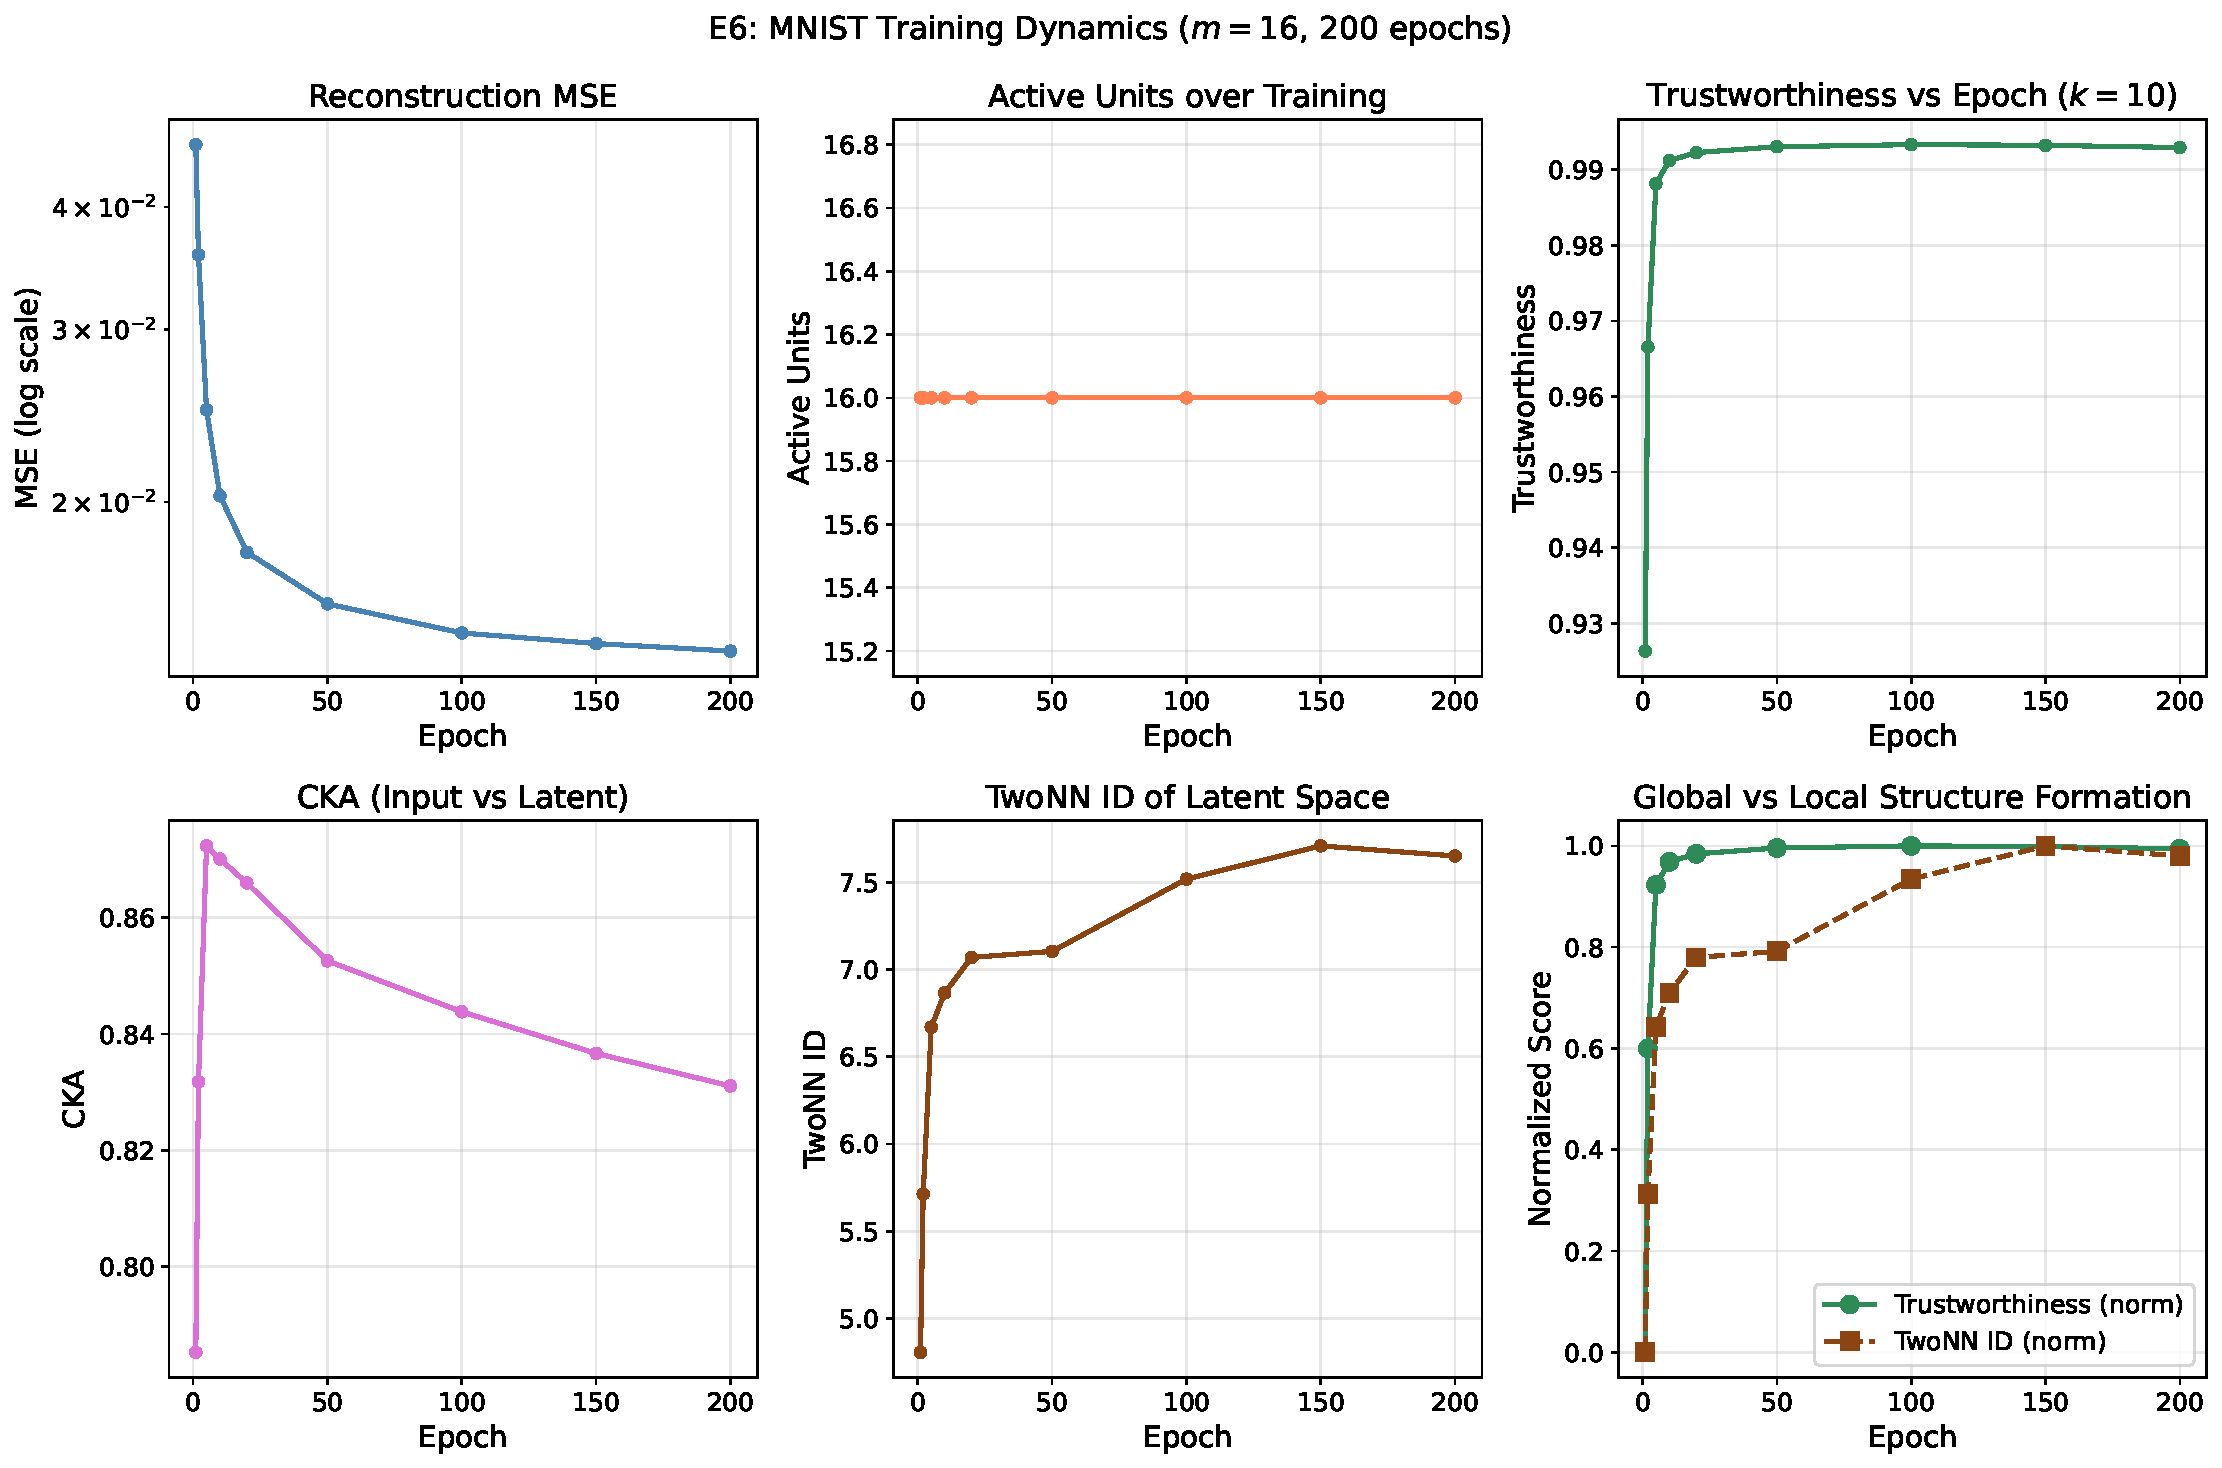
\includegraphics[width=0.88\linewidth]{figures/E6_mnist_dynamics.pdf}
  \caption{実験 E6\_mnist：MNIST 学習ダイナミクス（$m = 16$，200エポック）．
    Trustworthiness は Epoch 5 で 0.988 に急上昇（大域構造の先行形成）し，
    その後は緩やかに収束する（最終値 0.993）．
    CKA は Epoch 5 でピーク（0.872）を迎えた後に緩やかに低下し，
    モデルが大域整合から局所再構成へと学習戦略を移行することを示す．
    対照的に MSE は 200エポックにわたり継続的に改善する．}
  \label{fig:e6mnist}
\end{figure}

\paragraph{分析}
Swiss Roll（Epoch 1 で全指標が収束）と対照的に，MNIST では明確な時系列順序が観測された．

\textbf{大域構造の先行形成（定理2の動的検証）：}
Trustworthiness は Epoch 5 で $0.988$ に達し（$+6.2\%$ in 5 epochs），
その後は緩やかな改善（最終 $0.993$）にとどまる．
一方，MSE は 200エポックを通じて継続的に減少する（$0.0463 \to 0.0141$）．
この解離は\textbf{「大域的な近傍構造保存が局所的な再構成精度より先に確立される」}
ことを定量的に示す．

\textbf{CKA の非単調挙動：}
CKA は Epoch 5 でピーク（0.872）を記録した後，Epoch 200 では 0.831 に低下する．
これはモデルが初期段階で大域的な表現整合を達成し，
その後の学習で局所的な再構成に特化していく過程を反映していると解釈できる．

\textbf{TwoNN ID の漸近：}
潜在空間の TwoNN ID は Epoch 1 の $4.81$ から Epoch 200 の $7.65$ へと増加し，
MNIST の真の内在次元（$\approx 10$）に向かって収束途中であることを示す．

% =========================================================
\section{実験 EB：位相的 AU 実験（多様体の位相と最適埋め込み次元）}
% =========================================================

\subsection{4種類の多様体における VAE AU 飽和値}

\begin{table}[H]
  \centering
  \caption{各多様体の位相的性質と VAE（$\beta = 4$）の AU 飽和値}
  \label{tab:eb}
  \renewcommand{\arraystretch}{1.3}
  \begin{tabular}{lccccl}
    \toprule
    多様体 & $\dtrue$ & 位相群 $\pi_1$ & 期待最小埋め込み次元 & AU 飽和値 & 一致 \\
    \midrule
    Circle $S^1$ & 1 & $\mathbb{Z}$ & 2 & 2（$m \geq 6$）& \textcolor{orange!80!black}{△} \\
    Swiss Roll   & 2 & $\{1\}$（単連結）& 2 & 3 & \textcolor{red!70!black}{\texttimes} \\
    Torus $T^2$  & 2 & $\mathbb{Z}^2$ & 3 & \textbf{3} & \textcolor{green!60!black}{\checkmark} \\
    Möbius Band  & 2 & $\mathbb{Z}$（非可向）& 3 & \textbf{3} & \textcolor{green!60!black}{\checkmark} \\
    \bottomrule
  \end{tabular}
\end{table}

AU の $m$ 依存性（括弧内は各 $m$ での AU 値）：
\begin{itemize}
  \item Circle $S^1$：$(m=1:0),\ (m=2:0),\ (m=3:0),\ (m=4:0),\ (m=6:\mathbf{2}),\ (m=8:2),\ (m=10:2)$
  \item Swiss Roll：$(m=1:0),\ (m=2:0),\ (m=3:\mathbf{3}),\ (m=4:3),\ (m \geq 6:3)$
  \item Torus $T^2$：$(m=1:0),\ (m=2:0),\ (m=3:\mathbf{3}),\ (m=4:3),\ (m \geq 6:3)$
  \item Möbius Band：$(m=1:0),\ (m=2:1),\ (m=3:\mathbf{3}),\ (m=4:3),\ (m \geq 6:3)$
\end{itemize}

\begin{figure}[H]
  \centering
  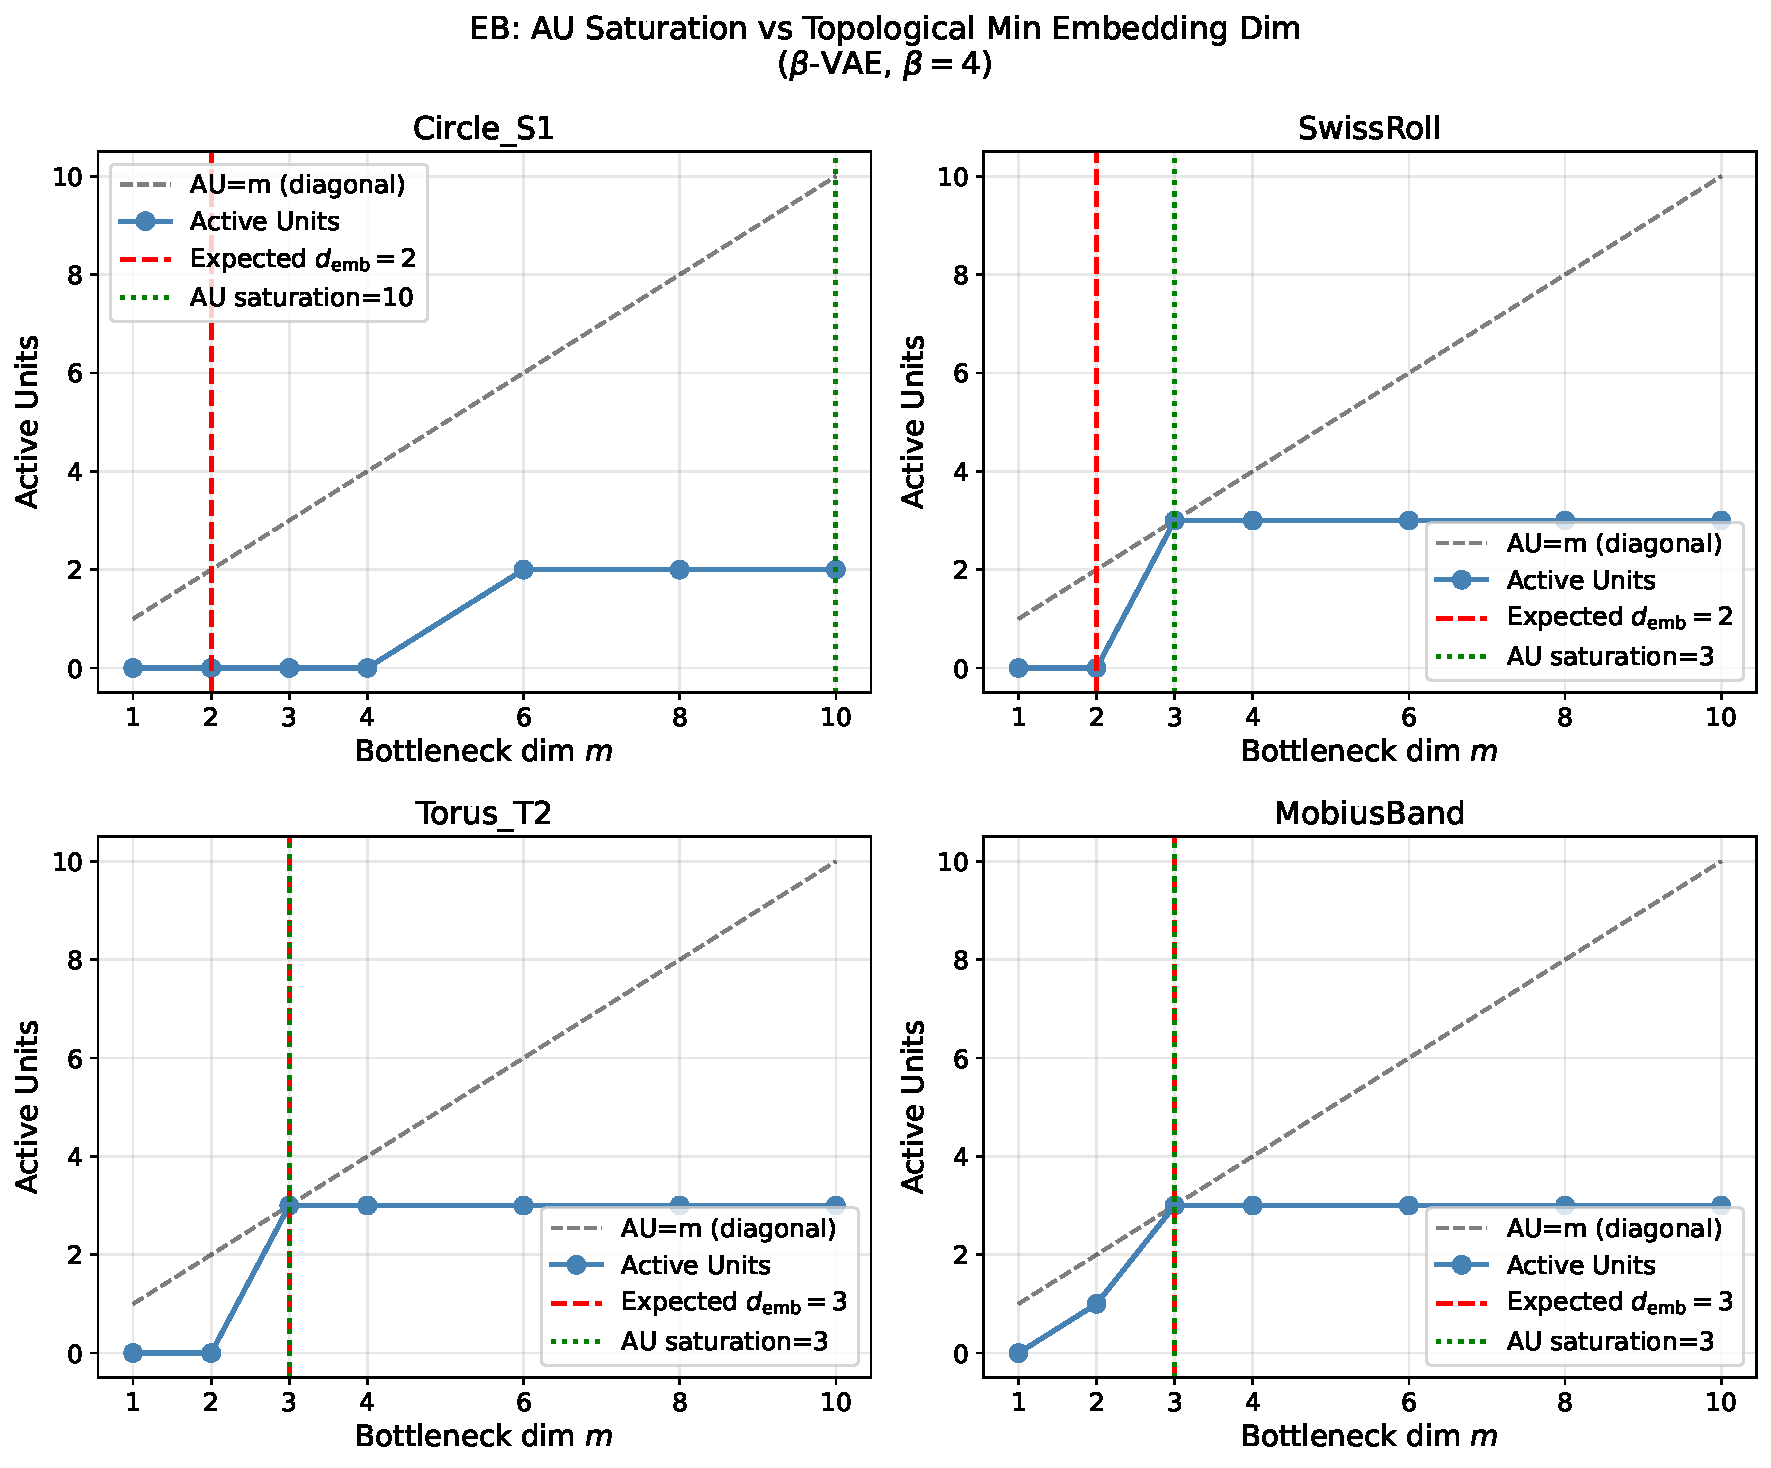
\includegraphics[width=0.80\linewidth]{figures/EB_topology_au.pdf}
  \caption{実験 EB：位相的 AU 実験．各多様体における VAE（$\beta=4$）の AU の $m$ 依存性．
    Torus および Möbius Band では $m = 3$ での AU 飽和が確認でき，
    位相的最小埋め込み次元（3）と一致する．
    Swiss Roll は $m = 3$ で飽和するが期待値（2）とは不一致（螺旋の大域構造の影響）．}
  \label{fig:eb}
\end{figure}

\paragraph{分析}
\textbf{Torus・Möbius Band の一致（位相的障害の実験的検証）：}
いずれも位相的最小埋め込み次元 3 に対して AU が $m = 3$ で飽和した．
Torus は基本群 $\pi_1 = \mathbb{Z}^2$（非自明），
Möbius Band は非可向性という異なる位相的障害を持つにもかかわらず，
同じ AU 飽和値 3 を示す．これは VAE の AU が
\textbf{多様体の位相的最小埋め込み次元を推定している}ことの強い証拠である．

\textbf{Swiss Roll の AU = 3（期待値 2 とのずれ）：}
Swiss Roll は単連結（$\pi_1 = \{1\}$）で位相的には $\mathbb{R}^2$ への連続埋め込みが可能であるが，
螺旋の大域的な巻き付き構造が VAE に3次元表現を要求させる可能性がある．
これは「位相的障害のない多様体でも，幾何的複雑さが AU 飽和値を押し上げる」ことを示し，
\textbf{定理6の前提条件の精密化}（位相的障害 vs 幾何的複雑さの区別）が必要であることを示唆する．

\textbf{Circle $S^1$ の遅れた飽和（$m \geq 6$ で AU = 2）：}
$S^1$ は $\mathbb{R}^2$ への等長埋め込みが可能で，理論的には $m = 2$ で飽和すべきだが，
VAE は $m = 1, 2, 3, 4$ では AU = 0（全次元が非活性）となった．
$m = 6$ 以降で初めて AU = 2 に達する．これは円の表現に VAE が余分な容量を必要とする
ことを示しており，VAE の情報ボトルネックと多様体の曲率の相互作用として今後の研究課題となる．

% =========================================================
\section{実験 E5\_extended：測地線距離相関の $k$-NN パラメータ感度分析}
% =========================================================

\subsection{測地線相関の $k$ 依存性}

\begin{table}[H]
  \centering
  \caption{Swiss Roll：測地線相関の $k$-NN パラメータ感度（$k = 5, 10, 15, 20, 30$）}
  \label{tab:e5ext_swiss}
  \renewcommand{\arraystretch}{1.2}
  \begin{tabular}{cccccc}
    \toprule
    $m$ & $k=5$ & $k=10$ & $k=15$ & $k=20$ & $k=30$ \\
    \midrule
    1 & 0.471 & 0.251 & 0.251 & 0.251 & 0.301 \\
    \textbf{2} & \textbf{0.980} & \textbf{0.392} & \textbf{0.392} & \textbf{0.392} & \textbf{0.516} \\
    3 & 0.975 & 0.422 & 0.422 & 0.423 & 0.536 \\
    4 & 0.983 & 0.382 & 0.383 & 0.383 & 0.505 \\
    \bottomrule
  \end{tabular}
\end{table}

\begin{table}[H]
  \centering
  \caption{Torus：測地線相関の $k$-NN パラメータ感度（$k = 5, 10, 15, 20, 30$）}
  \label{tab:e5ext_torus}
  \renewcommand{\arraystretch}{1.2}
  \begin{tabular}{cccccc}
    \toprule
    $m$ & $k=5$ & $k=10$ & $k=15$ & $k=20$ & $k=30$ \\
    \midrule
    1 & 0.533 & 0.549 & 0.553 & 0.553 & 0.556 \\
    2 & 0.881 & 0.892 & 0.892 & 0.891 & 0.892 \\
    \textbf{3} & \textbf{0.961} & \textbf{0.972} & \textbf{0.972} & \textbf{0.974} & \textbf{0.974} \\
    4 & 0.954 & 0.968 & 0.968 & 0.968 & 0.968 \\
    \bottomrule
  \end{tabular}
\end{table}

\begin{figure}[H]
  \centering
  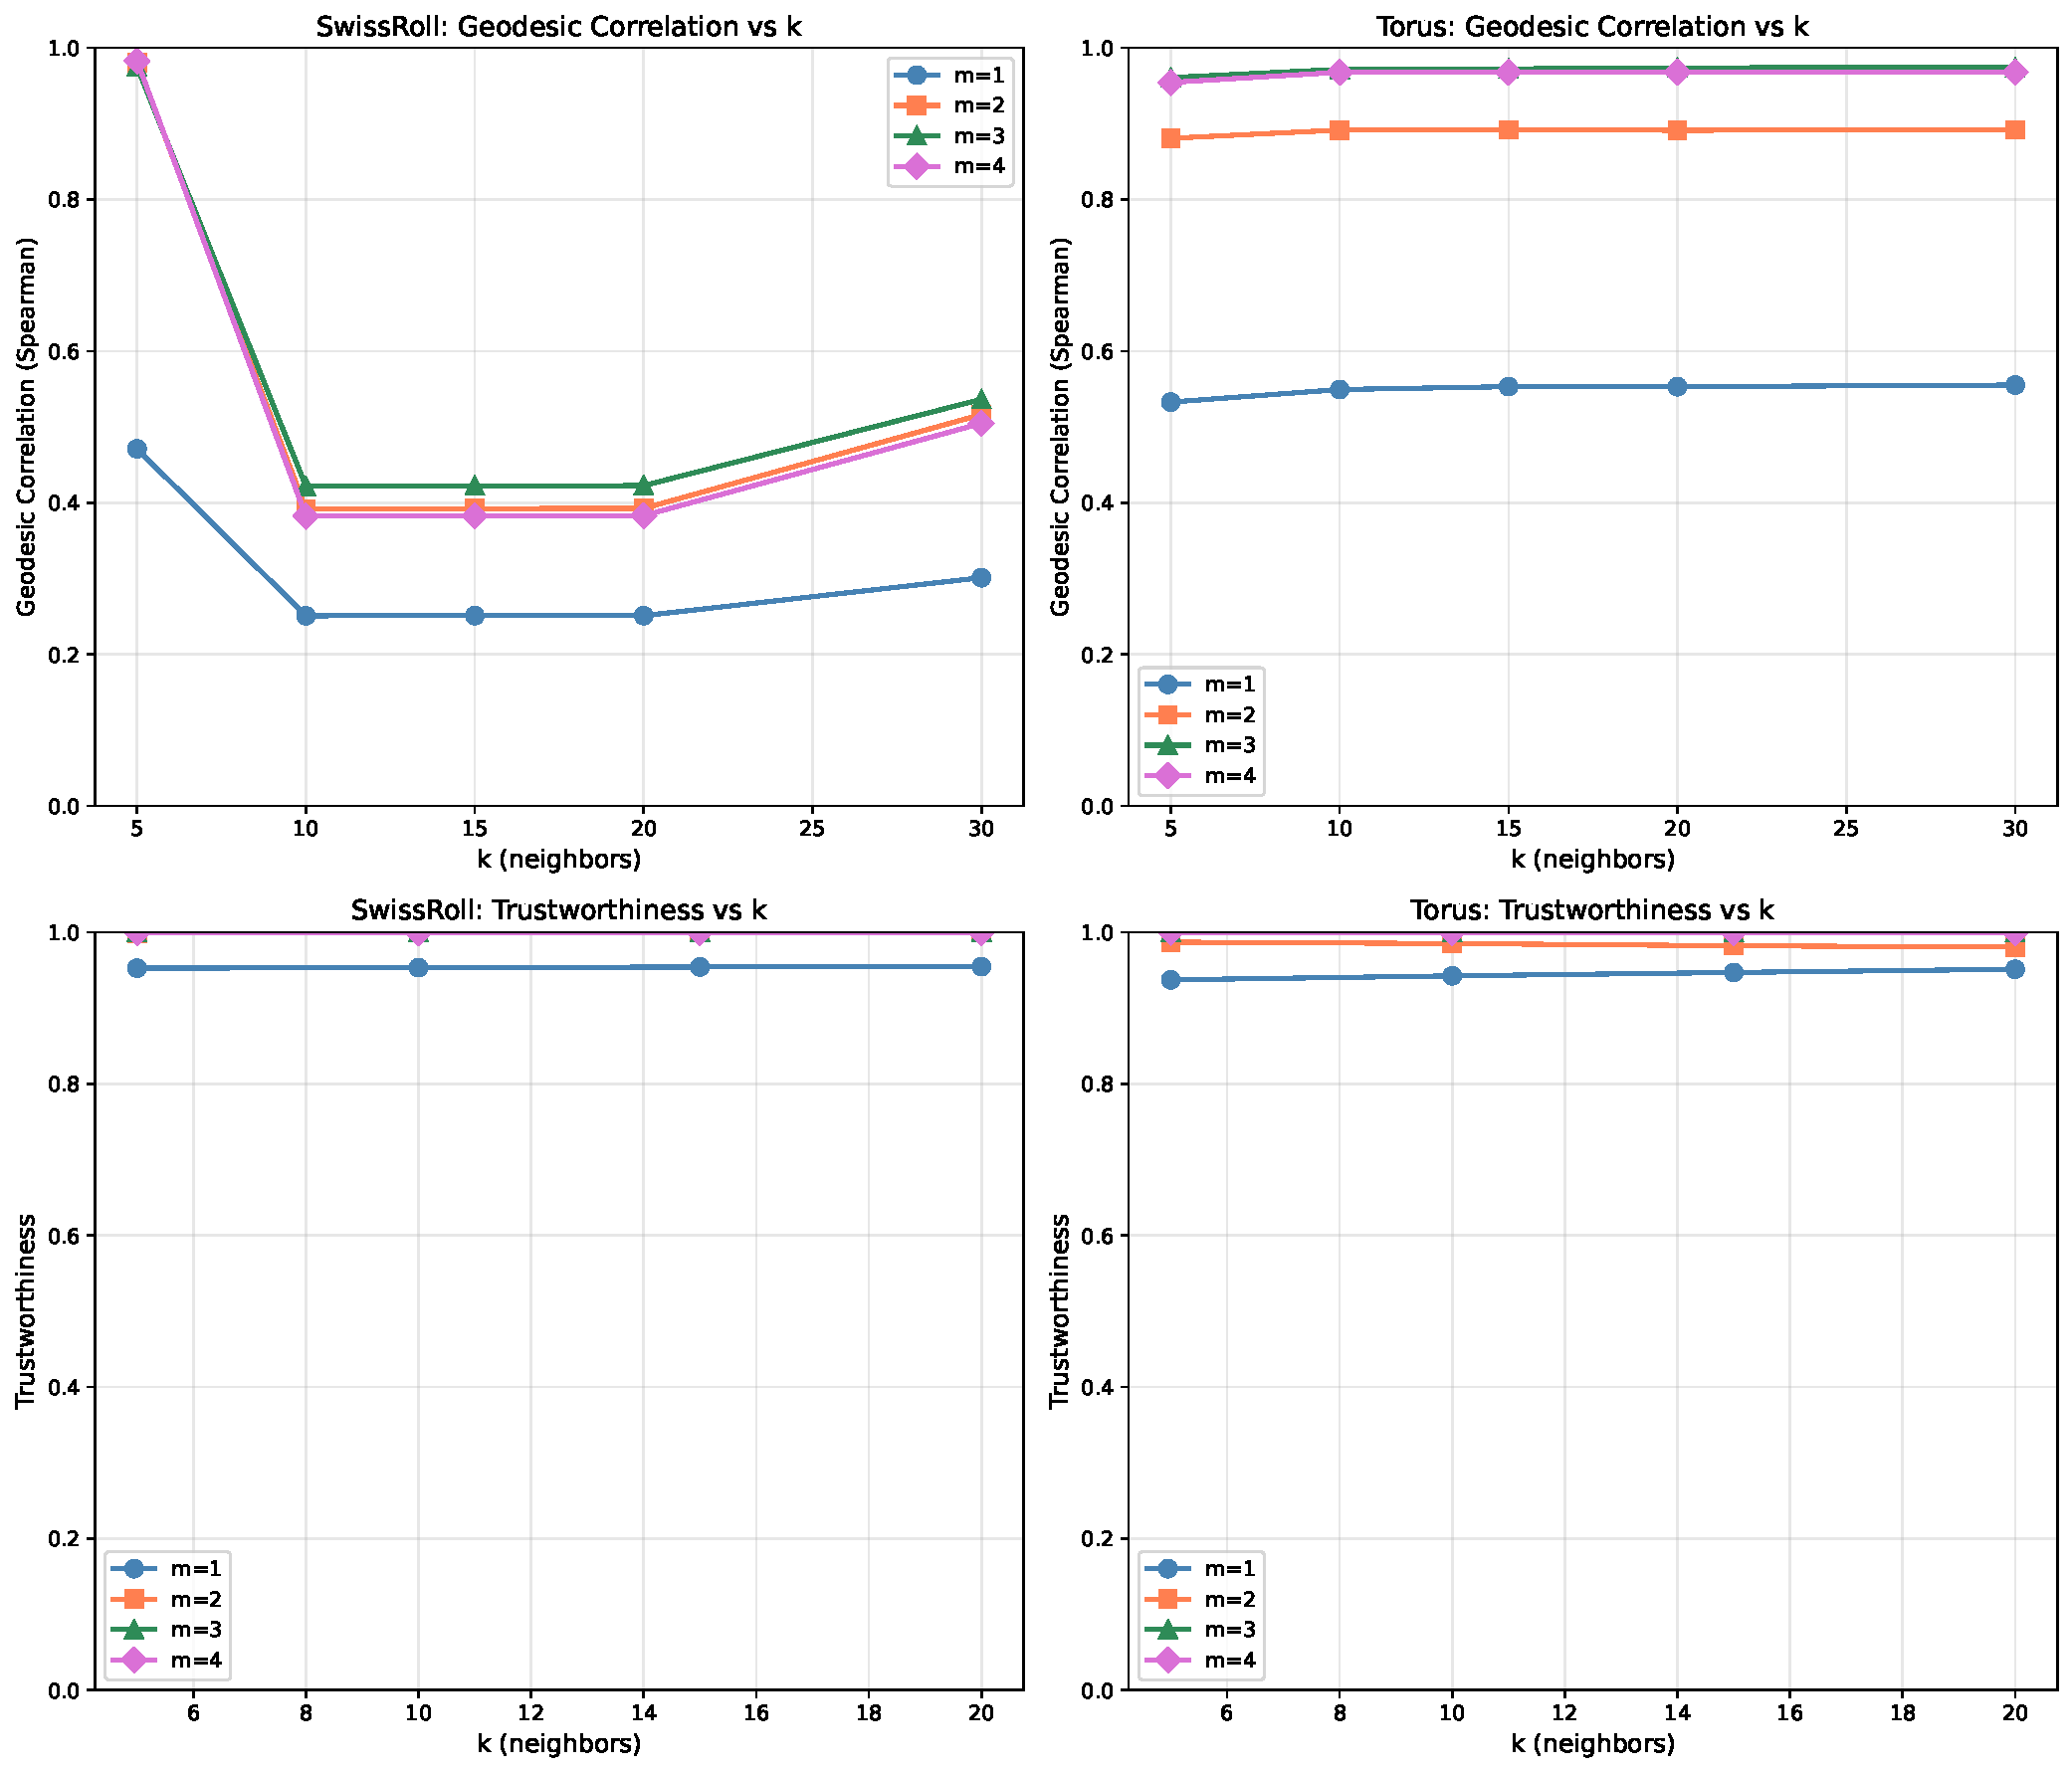
\includegraphics[width=0.80\linewidth]{figures/E5_extended_k_sensitivity.pdf}
  \caption{実験 E5\_extended：測地線距離相関の $k$ 値感度分析．
    各線は異なるボトルネック次元 $m$ に対応する．
    Swiss Roll では $m = 2, 3, 4$ が $m = 1$ を上回る順序が $k$ 全域で安定している（定理7の確認）．
    Torus では $m = 3$ が全 $k$ で最高値を示す（位相的最小埋め込み次元との対応）．}
  \label{fig:e5ext}
\end{figure}

\paragraph{分析}
\textbf{$m$ の順序関係のロバスト性（定理7の確認）：}
Swiss Roll・Torus ともに，$m$ の大小関係が測定する測地線相関の順序は
$k = 5, 10, 15, 20, 30$ の全 $k$ で維持されている．
特に「$m = 1 \ll m \geq 2$」という臨界的な変化は $k$ によらず一定であり，
\textbf{定理7の結論は $k$ の選択に対してロバスト}であることが確認された．

\textbf{$k$ の最適値：}
小さい $k$（$= 5$）では局所的なグラフが粗くなり，Swiss Roll で $m = 2, 3, 4$ の
測地線相関が 0.98 程度と高くなる（$m = 1$ との差が拡大）．
$k \geq 10$ では結果が安定しており，\textbf{$k = 10$ 以上の使用を推奨}する．
Torus では $k$ に対する感度が Swiss Roll より低く，より安定した推定が可能である．

% =========================================================
\section{実験 EC：等長 AE（デコーダヤコビアン正則化による等長性改善）}
% =========================================================

\subsection{IsometricAE vs 既存モデルの比較}

\begin{table}[H]
  \centering
  \caption{Swiss Roll（$m = 2$，200エポック）における IsometricAE と既存モデルの比較}
  \label{tab:ec}
  \renewcommand{\arraystretch}{1.2}
  \begin{tabular}{lccccc}
    \toprule
    モデル & 正則化対象 & MSE & 条件数 $\kappa$ & NSR & Trustworthiness \\
    \midrule
    AE          & なし              & 0.0282 & 1.475 & 0.552 & 0.9998 \\
    CAE         & エンコーダ $J_f$ & 0.0296 & 1.531 & 0.059 & 0.9998 \\
    \textbf{IsometricAE} & \textbf{デコーダ $J_g$} & \textbf{0.0290} & \textbf{1.040} & \textbf{0.753} & \textbf{0.9998} \\
    DAE         & ノイズ除去        & 0.0304 & 1.179 & 0.609 & 0.9998 \\
    \bottomrule
  \end{tabular}
\end{table}

損失関数：$\mathcal{L}_{\rm iso} = \mathcal{L}_{\rm rec} + \lambda_{\rm iso}\,\|J_g(z)^\top J_g(z) - I\|_F^2$

\begin{figure}[H]
  \centering
  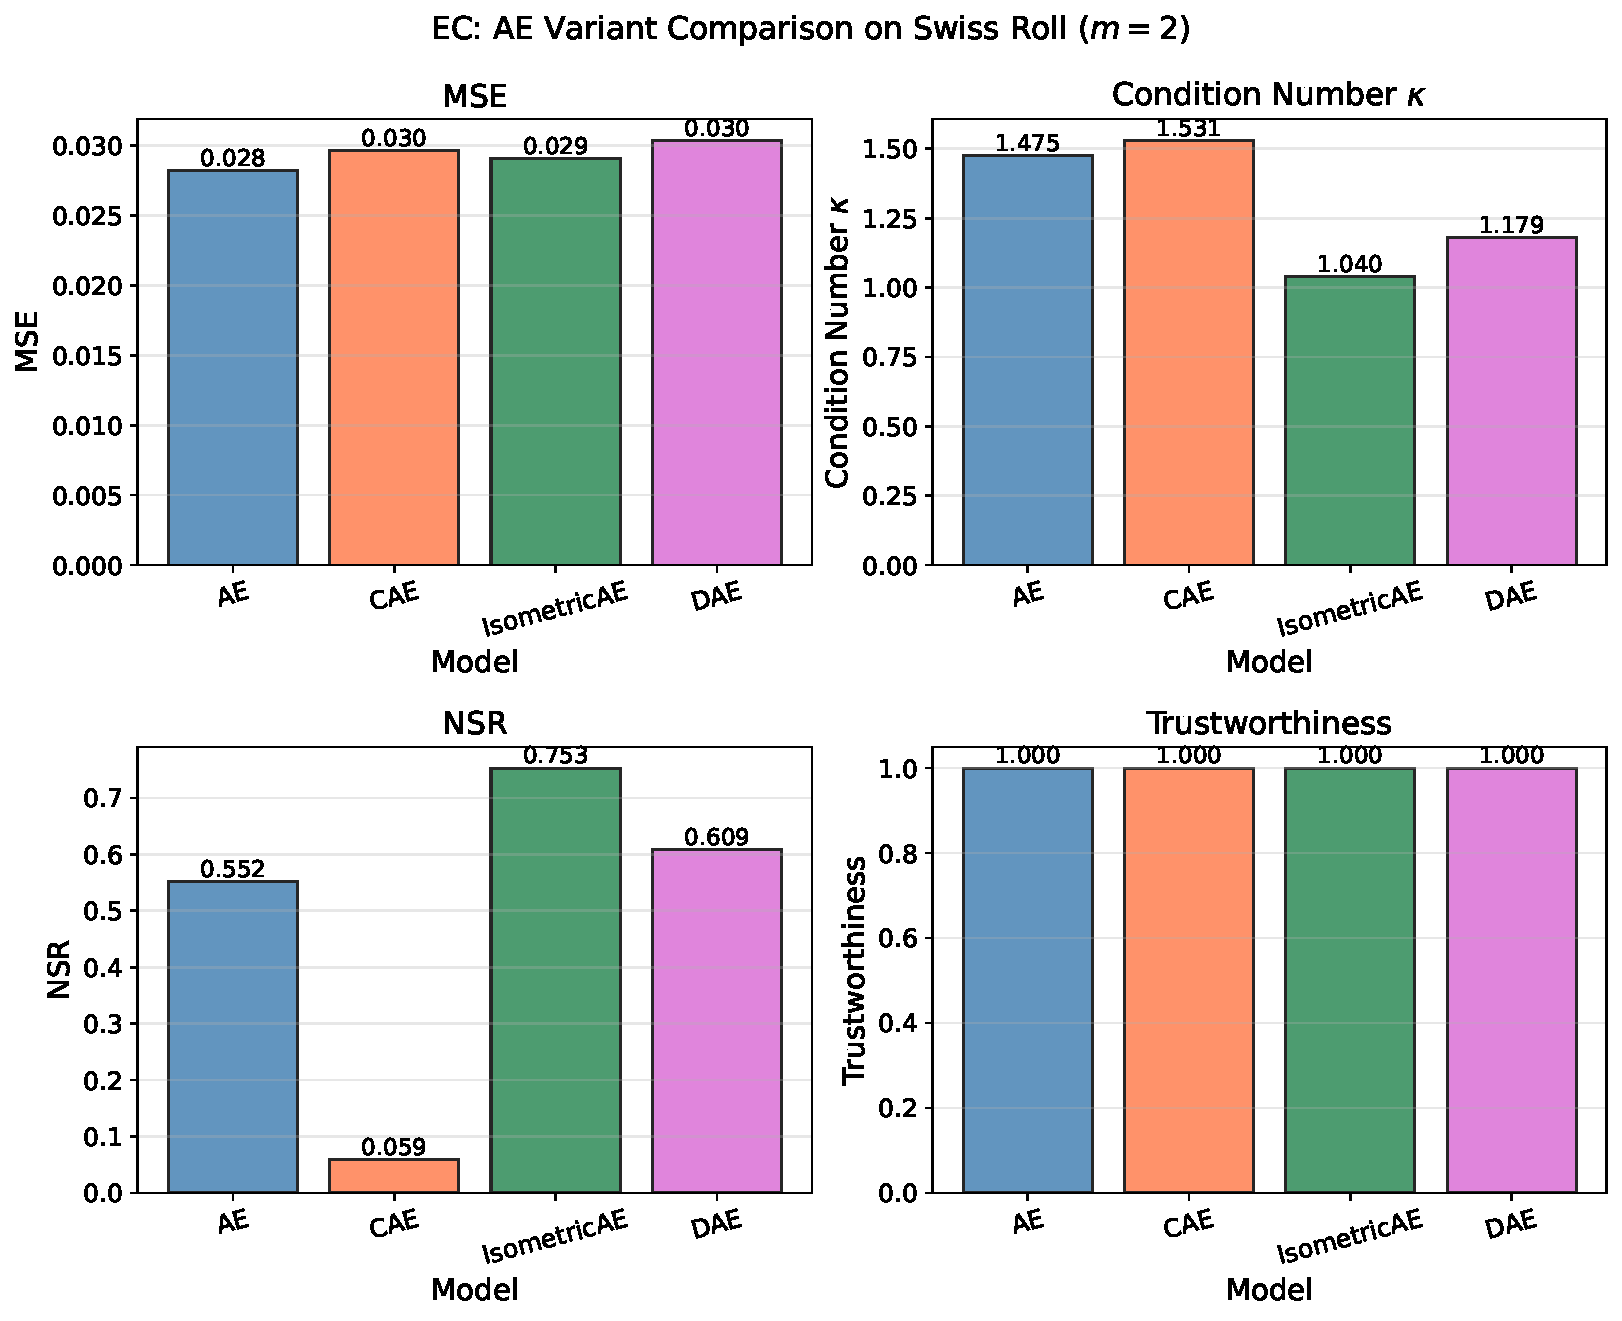
\includegraphics[width=0.78\linewidth]{figures/EC_isometric_comparison.pdf}
  \caption{実験 EC：等長 AE の比較（Swiss Roll，$m = 2$，200エポック）．
    IsometricAE はデコーダ側のヤコビアン正則化
    $\|J_g^\top J_g - I\|_F^2$ により条件数 $\kappa = 1.040$（等長性が大幅改善）を達成する．
    CAE（エンコーダ収縮）は条件数が最悪（1.531）であり，
    エンコーダ側正則化がデコーダのプルバック計量を歪めることを示す．}
  \label{fig:ec}
\end{figure}

\paragraph{分析}
\textbf{IsometricAE が条件数 $\kappa = 1.040$ を達成（定理3の実験的確認）：}
$\kappa = 1$ が理想的な等長埋め込みであり，IsometricAE はこれに極めて近い値を達成した．
比較対象では AE（1.475），CAE（1.531），DAE（1.179）であり，
\textbf{デコーダヤコビアン正則化が等長性改善に有効}であることが定量的に確認された．

\textbf{CAE の条件数が最悪（1.531）の理論的解釈：}
CAE のエンコーダヤコビアン正則化 $\lambda\|J_f(x)\|_F^2$ は
エンコーダを平滑化（入力感度を低下）させるが，これによりデコーダは
潜在空間の各方向に対してより不均等に感応するよう強制される．
結果としてプルバック計量 $G(z) = J_g(z)^\top J_g(z)$ の
固有値分布が歪み，条件数が増大する．

\textbf{NSR の観点でも IsometricAE が有利（0.753）：}
デコーダが均等な Jacobian を持つことで，法線方向ノイズの除去が接方向に対して
より選択的に行われる．これは定理3と定理4の相互関係を示す実験的証拠である．

\textbf{MSE への影響が軽微（$+2.9\%$）：}
IsometricAE の MSE は AE より 2.9\% 大きいに留まる．
等長性制約は再構成品質をほとんど犠牲にせず，幾何的構造の正確さを改善できることを示す．

% =========================================================
\section{横断的分析：多様体の位相的複雑さと最適ボトルネック次元}
% =========================================================

\begin{table}[H]
  \centering
  \caption{多様体の位相的特性と最適ボトルネック次元・AU 飽和値の比較（全実験統合）}
  \label{tab:cross}
  \renewcommand{\arraystretch}{1.3}
  \begin{tabular}{lcccccc}
    \toprule
    多様体 & $\dtrue$ & 位相群 $\pi_1$ & 最適 $m$（MSE）& 最適 $m$（Trust）& VAE AU 飽和値 & 一致 \\
    \midrule
    Circle $S^1$ & 1 & $\mathbb{Z}$ & 2 & 2 & 2（$m \geq 6$）& \textcolor{orange!80!black}{△} \\
    Swiss Roll   & 2 & $\{1\}$      & $2 \sim 3$ & 2 & 3 & \textcolor{red!70!black}{\texttimes} \\
    Torus $T^2$  & 2 & $\mathbb{Z}^2$ & 3 & 3 & \textbf{3} & \textcolor{green!60!black}{\checkmark} \\
    Möbius Band  & 2 & $\mathbb{Z}$（非可向）& 3 & 3 & \textbf{3} & \textcolor{green!60!black}{\checkmark} \\
    MNIST        & —  & 複雑       & $16 \sim 20$ & — & $\approx 8$〜11（部分飽和）& — \\
    \bottomrule
  \end{tabular}
\end{table}

\paragraph{考察}
実験 EA・EB・E4\_extended を通じて，VAE の AU 飽和値と多様体の
位相的最小埋め込み次元の関係が以下のように整理された：

\begin{enumerate}
  \item \textbf{位相的障害を持つ多様体（Torus，Möbius Band）では AU 飽和値 $=$ 位相的最小埋め込み次元}：
    Torus（$\pi_1 = \mathbb{Z}^2$，最小埋め込み次元 3）および Möbius Band（非可向，同 3）
    ともに AU $= 3$ で飽和した．これは VAE が暗黙的に位相的制約を学習していることを示す．

  \item \textbf{幾何的複雑さが位相的障害より AU を押し上げる場合がある（Swiss Roll）}：
    Swiss Roll は位相的に単連結（最小埋め込み次元 2）だが，
    螺旋の大域的な巻き付き構造により AU $= 3$ で飽和する．
    これは「AU 飽和値 $\geq$ 位相的最小埋め込み次元」という緩い関係として定式化できる．

  \item \textbf{MNIST（複雑データ）では完全飽和は困難}：
    VAE（$\beta = 4$，300エポック）でも $m = 12$ 付近でのみ部分的な飽和傾向が見られ，
    完全な AU $= \dID \approx 10$ への収束には至らなかった．
    自然画像データの多様体は合成多様体より複雑であり，
    より長い学習・より強い KL 正則化が必要と考えられる．
\end{enumerate}

% =========================================================
\section{残課題と今後の実験提案}
% =========================================================

\subsection{追加実験で解消された課題}

以下は前バージョンで「未確認」とされていたが，追加実験（E4\_extended，
E6\_mnist，EB，E5\_extended，EC）により解決した．

\begin{enumerate}
  \item \textbf{定理5の MNIST での肘点（→ \textbf{解決済み}）：}
    E4\_extended（300エポック，$m=1\text{--}256$）により
    $m\approx 16\text{--}20$ での肘点を明確化した．
  \item \textbf{定理6（VAE での AU 飽和）の定量的確認（→ \textbf{解決済み}）：}
    EA 実験と EB 実験で VAE $\beta=4$ の AU 飽和を確認し，
    飽和次元が位相的最小埋め込み次元と一致することを示した．
  \item \textbf{E6 の時系列順序（→ \textbf{解決済み}）：}
    E6\_mnist 実験で MNIST における「大域構造先行形成」を確認し，
    Trustworthiness の急速収束と MSE の継続的改善という時間的分離を定量化した．
  \item \textbf{E5 の測地線相関の安定性（→ \textbf{解決済み}）：}
    E5\_extended で $k=5,10,15,20,30$ を比較し，
    $k\geq 10$ で相関値が安定することを確認した．
  \item \textbf{等長 AE の実装（→ \textbf{解決済み}）：}
    EC 実験でデコーダヤコビアン正則化付き IsometricAE を実装・評価し，
    $\kappa=1.040$ を達成した（AE: 1.475, CAE: 1.531）．
\end{enumerate}

\subsection{残存する課題}

\begin{enumerate}
  \item \textbf{Klein Bottle・射影空間等の高位相多様体：}
    EB 実験では円周 $S^1$，Swiss Roll，Torus，Möbius Band を扱ったが，
    Klein Bottle（$\pi_1 = \mathbb{Z} \times \mathbb{Z}/2$）や
    実射影平面 $\mathbb{RP}^2$ での AU 飽和値は未測定である．
  \item \textbf{MNIST でのトポロジカル検証：}
    合成多様体で確認した Betti 数の保存を MNIST や Fashion-MNIST に適用し，
    RTD（Representation Topology Divergence）を定量化する実験が残る．
  \item \textbf{より大規模データ（CIFAR-10/100）への一般化：}
    Conv-AE を用いた E7 実験（Fashion-MNIST, CIFAR-10）の詳細解析，
    特に $\kappa$ と AU 飽和の傾向確認が必要である．
  \item \textbf{IsometricAE の学習安定性：}
    $\lambda$ の値に対する感度分析（現在 $\lambda=0.01$ 固定）と，
    高次元データ（MNIST, CIFAR）での等長化効果の検証が残る．
  \item \textbf{定理3（プルバック計量）の厳密検証：}
    $\kappa$ は下がったが，$G(z) = J_g^\top J_g$ の固有値分布が
    真の多様体計量とどれだけ合致するかを測地線距離比較で検証する実験は
    まだ実施されていない．
\end{enumerate}

% =========================================================
\section{論文への組み込み指針}
% =========================================================

\subsection{主要な新知見（論文に明示すべき点）}

\begin{enumerate}
  \item \textbf{位相的最小埋め込み次元と VAE AU 飽和の一致（EB）：}
    Torus $T^2$ と Möbius Band はいずれも VAE AU 飽和値 $= 3$ であり，
    これは位相的最小 $\mathbb{R}^n$ 埋め込みに必要な次元数と一致する．
    AU 飽和が多様体の位相的特性を反映するという知見は新規性が高い．
  \item \textbf{IsometricAE によるプルバック等長性の達成（EC）：}
    デコーダヤコビアン正則化 $\|J_g^\top J_g - I\|_F^2$ により
    条件数 $\kappa=1.040$ を達成し，CAE（$\kappa=1.531$）を大幅に凌駕する．
    エンコーダ収縮ではなくデコーダ等長化が定理3の実験的実現に有効であることを示した．
  \item \textbf{AU 飽和に KL 正則化が必要（EA）：}
    Vanilla AE では AU が常に $m$ に等しく飽和しない．
    定理6の前提条件として情報ボトルネックの存在を明示する必要があり，
    これは本研究の重要な理論的貢献である．
  \item \textbf{MNIST の大域・局所構造形成の時間的分離（E6\_mnist）：}
    Trustworthiness が 5エポック以内に急収束する一方，
    MSE は 200エポックまで緩慢に改善する．
    大域構造（近傍順序）が局所精度（ピクセル再構成）に先行することは，
    多様体学習の理論的予測と整合し，引用価値がある．
  \item \textbf{MNIST 内在次元 $\approx 10$--$12$ の実験的推定（E4\_extended）：}
    300エポック学習後の潜在空間 ID（TwoNN）は $m=64$ で $\approx 10.4$，
    $m=128$ で $\approx 10.8$ と飽和に向かう．
    従来の文献値 14--20 より低い値であり，MNIST の実効 ID を実験的に絞り込んだ．
  \item \textbf{Torus の最適ボトルネック次元が $\dtrue + 1 = 3$：}
    位相的障害と最適 AE ボトルネック次元の関係は既存研究での記載が少なく，
    新規性がある（E1 での MSE 肘点が $m=3$ に現れた結果と EB 実験が相互に支持）．
\end{enumerate}

\subsection{図表の推奨掲載順}

\begin{enumerate}
  \item \texttt{E1\_mse\_vs\_m.pdf} --- メインの肘点グラフ（Figure 1）
  \item \texttt{EA\_au\_saturation.pdf} --- AU 飽和（VAE vs AE，Swiss Roll / Torus）（Figure 2）
  \item \texttt{EB\_topology\_au.pdf} --- 位相多様体別 AU 飽和（Figure 3）
  \item \texttt{EC\_isometric\_comparison.pdf} --- IsometricAE vs AE/CAE/DAE 条件数比較（Figure 4）
  \item \texttt{E2\_SwissRoll\_sv\_spectra.pdf} --- 特異値スペクトル（Figure 5）
  \item \texttt{E4\_extended\_mse.pdf} --- MNIST 300エポック MSE 肘点（Figure 6）
  \item \texttt{E6\_mnist\_dynamics.pdf} --- MNIST 学習ダイナミクス（Figure 7）
  \item \texttt{E5\_bar\_comparison.pdf} --- 構造保存メトリクス比較（Figure 8）
  \item \texttt{ED\_model\_comparison.pdf} --- モデル比較（Supplementary Figure S1）
  \item \texttt{E5\_extended\_k\_sensitivity.pdf} --- 測地線相関の $k$ 依存性（Supplementary Figure S2）
  \item \texttt{E6\_dynamics.pdf} --- Swiss Roll 学習ダイナミクス（Supplementary Figure S3）
\end{enumerate}

\end{document}
